%% Template for the submission to:
%%   The Annals of Applied Statistics [AOAS]
%%
%%%%%%%%%%%%%%%%%%%%%%%%%%%%%%%%%%%%%%%%%%%%%%
%% In this template, the places where you   %%
%% need to fill in your information are     %%
%% indicated by '???'.                      %%
%%                                          %%
%% Please do not use \input{...} to include %%
%% other tex files. Submit your LaTeX       %%
%% manuscript as one .tex document.         %%
%%%%%%%%%%%%%%%%%%%%%%%%%%%%%%%%%%%%%%%%%%%%%%

\documentclass[aoas]{imsart}

%% Packages
\RequirePackage{amsthm,amsmath,amsfonts,amssymb}
\RequirePackage[authoryear]{natbib}
\RequirePackage[colorlinks,citecolor=blue,urlcolor=blue]{hyperref}%% uncomment this for coloring bibliography citations and linked URLs
\RequirePackage{graphicx}%% uncomment this for including figures



%%PACKAGES
\usepackage{caption}
\usepackage{subcaption}
\usepackage{float}
\usepackage{multirow}
\usepackage{lscape}
\usepackage{calc}
\usepackage{array}
\usepackage{bbold}
\usepackage{comment}
\usepackage{xcolor}
\usepackage{nicematrix}
\usepackage{multirow}
\usepackage{diagbox}
\usepackage{tikz}
\usepackage{yhmath}
\usetikzlibrary{quotes,angles}
\usepackage{pgfplots}
\pgfplotsset{compat = newest}
\usepackage{fancyhdr}


% set up for custom R code
\usepackage{listings}
\definecolor{darkgreen}{rgb}{0.0, 0.5, 0.0} % Define a dark green color for the comments

\lstdefinestyle{customR}{
	language=R,
	backgroundcolor=\color{lightgray},
	basicstyle=\ttfamily\footnotesize,
	keywordstyle=\bfseries\color{blue},
	commentstyle=\itshape\color{darkgreen}, % Use the custom dark green color
	stringstyle=\color{red},
	numbers=left,
	numberstyle=\tiny\color{gray},
	stepnumber=1,
	numbersep=10pt,
	showspaces=false,
	showstringspaces=false,
	showtabs=false,
	frame=single,
	rulecolor=\color{black},
	tabsize=2,
	captionpos=b,
	breaklines=true,
	breakatwhitespace=false,
	title=\lstname,
	escapeinside={\%*}{*)},
	morekeywords={*,...} % if you want to add more keywords to highlight
}

\lstset{style=customR}


\startlocaldefs
%%%%%%%%%%%%%%%%%%%%%%%%%%%%%%%%%%%%%%%%%%%%%%
%%                                          %%
%% Uncomment next line to change            %%
%% the type of equation numbering           %%
%%                                          %%
%%%%%%%%%%%%%%%%%%%%%%%%%%%%%%%%%%%%%%%%%%%%%%
%\numberwithin{equation}{section}
%%%%%%%%%%%%%%%%%%%%%%%%%%%%%%%%%%%%%%%%%%%%%%
%%                                          %%
%% For Axiom, Claim, Corollary, Hypothesis, %%
%% Lemma, Theorem, Proposition              %%
%% use \theoremstyle{plain}                 %%
%%                                          %%
%%%%%%%%%%%%%%%%%%%%%%%%%%%%%%%%%%%%%%%%%%%%%%
%\theoremstyle{plain}
%\newtheorem{???}{???}
%\newtheorem*{???}{???}
%\newtheorem{???}{???}[???]
%\newtheorem{???}[???]{???}
%%%%%%%%%%%%%%%%%%%%%%%%%%%%%%%%%%%%%%%%%%%%%%
%%                                          %%
%% For Assumption, Definition, Example,     %%
%% Notation, Property, Remark, Fact         %%
%% use \theoremstyle{remark}                %%
%%                                          %%
%%%%%%%%%%%%%%%%%%%%%%%%%%%%%%%%%%%%%%%%%%%%%%
%\theoremstyle{remark}
%\newtheorem{???}{???}
%\newtheorem*{???}{???}
%\newtheorem{???}{???}[???]
%\newtheorem{???}[???]{???}
%%%%%%%%%%%%%%%%%%%%%%%%%%%%%%%%%%%%%%%%%%%%%%
%% Please put your definitions here:        %%

\newtheorem{theorem}{Theorem}[section]
\newtheorem{corollary}{Corollary}[section]
\newtheorem{lemma}{Lemma}[section]
\newtheorem{proposition}{Proposition}[section]

\theoremstyle{definition}
\newtheorem{definition}{Definition}[section]

\theoremstyle{remark}
\newtheorem*{remark}{Remark}
\theoremstyle{remark}
\newtheorem*{example}{Example}

%% SHORTCUTS
\DeclareMathOperator{\diag}{diag}
\DeclareMathOperator{\Span}{span}
\DeclareMathOperator{\erf}{erf}
\newcommand {\R}{\mathbb{R}}
\newcommand {\E}{\mathbb{E}}
\newcommand {\prob}{\mathbb{P}}
\newcommand {\N}{\mathbb{N}}
\newcommand {\Z}{\mathbb{Z}}
\newcommand {\1}{\mathbb{1}}


%%%%%%%%%%%%%%%%%%%%%%%%%%%%%%%%%%%%%%%%%%%%%%

\endlocaldefs

\begin{document}

\begin{frontmatter}
%%%%%%%%%%%%%%%%%%%%%%%%%%%%%%%%%%%%%%%%%%%%%%
%%                                          %%
%% Enter the title of your article here     %%
%%                                          %%
%%%%%%%%%%%%%%%%%%%%%%%%%%%%%%%%%%%%%%%%%%%%%%
\title{Varying coefficients correlated velocity models in complex landscapes with boundaries applied to narwhal responses to noise exposure}
%\title{A sample article title with some additional note\thanksref{T1}}
\runtitle{Movement models in complex landscapes}
%\thankstext{T1}{A sample of additional note to the title.}

\begin{aug}
%%%%%%%%%%%%%%%%%%%%%%%%%%%%%%%%%%%%%%%%%%%%%%%
%% Only one address is permitted per author. %%
%% Only division, organization and e-mail is %%
%% included in the address.                  %%
%% Additional information can be included in %%
%% the Acknowledgments section if necessary. %%
%% ORCID can be inserted by command:         %%
%% \orcid{0000-0000-0000-0000}               %%
%%%%%%%%%%%%%%%%%%%%%%%%%%%%%%%%%%%%%%%%%%%%%%%
\author[A]{\fnms{Alexandre}~\snm{Delporte}\ead[label=e1]{alexandre.delporte@univ-grenoble-alpes.fr}},
\author[B]{\fnms{Susanne}~\snm{Ditlevsen}\ead[label=e2]{susanne@math.ku.dk}}
\and
\author[A]{\fnms{Adeline}~\snm{Samson}\ead[label=e3]{adeline.leclercq-samson@univ-grenoble-alpes.fr}}
%%%%%%%%%%%%%%%%%%%%%%%%%%%%%%%%%%%%%%%%%%%%%%
%% Addresses                                %%
%%%%%%%%%%%%%%%%%%%%%%%%%%%%%%%%%%%%%%%%%%%%%%
\address[A]{Laboratoire Jean Kuntzmann,
	Université Grenoble-Alpes\printead[presep={,\ }]{e1,e3}}

\address[B]{Department of Mathematical Sciences,
	University of Copenhagen \printead[presep={,\ }]{e2}}
\end{aug}

\begin{abstract}
Narwhals in the Arctic are increasingly exposed to human activities that can temporarily or permanently threaten their survival by modifying their behavior. We examine GPS data from a population of narwhals exposed to ship and seismic airgun noise during a controlled experiment in 2018 in the Scoresby Sound fjord system in Southeast Greenland. The fjord system has a complex shore line, restricting the behavioral response options for the narwhals to escape the threats. We propose a new continuous-time correlated velocity model with varying coefficients that includes spatial constraints by adjusting the direction of the movement to the boundary of the domain. To assess the sound exposure effect we compare a baseline model for the movement before exposure to a response model for the movement during exposure. Our model, applied to the narwhal data, indicates that sound exposure can disturb motion up to a couple of tens of kilometers. Specifically, we found an increase in velocity and a decrease in persistence. We give estimates and confidence intervals of threshold distances to the sound source for medium and strong shifts in the whales motion.
\end{abstract}

\begin{keyword}
\kwd{behavioral response study}
\kwd{stochastic differential equations}
\kwd{mixed effect model}
\end{keyword}

\end{frontmatter}
%%%%%%%%%%%%%%%%%%%%%%%%%%%%%%%%%%%%%%%%%%%%%%
%% Please use \tableofcontents for articles %%
%% with 50 pages and more                   %%
%%%%%%%%%%%%%%%%%%%%%%%%%%%%%%%%%%%%%%%%%%%%%%
%\tableofcontents

%%%%%%%%%%%%%%%%%%%%%%%%%%%%%%%%%%%%%%%%%%%%%%
%%%% Main text entry area:

\section{Introduction}

%IN THIS DOCUMENT YOU SHOULD DO ALL CHANGES. YOU CAN JUST DO THEM DIRECTLY. IF YOU REMOVE THE \% SIGN FROM THE FILE latexmkrc YOU WILL SEE THE CLEAN DOCUMENT. WHAT IS ADDED IS COLORED BLUE, WHAT IS REMOVED IS RED AND STRIKED OVER.


%general context

%the models we consider
In ecology, animal movement is often modeled using continuous-time processes defined as solutions to stochastic differential equations (SDEs). One well-known example is the continuous-time correlated random walk, also called the integrated Ornstein-Uhlenbeck or correlated velocity model (CVM) \citep{johnson_continuous_2008}. It can be viewed as a special case of velocity potential model, where the potential is a second degree polynomial \citep{preisler_analyzing_2013}.  Varieties of CVMs have been applied to birds \citep{janaswamy_state_2018}, marine algae \citep{gurarie_estimating_2011}, ants \citep{russell_spatially_2018}, seals \citep{johnson_continuous_2008,albertsen_generalizing_2018}, bowhead whales \citep{gurarie_correlated_2017} and sea lion motion \citep{hanks_reflected_2017}.
In many cases, animal movement is assumed to occur without spatial constraints \citep{johnson_continuous_2008,michelot_varying-coefficient_2021,gurarie_correlated_2017}, though most animals encounter physical barriers during their locomotion. Ignoring such constraints can lead to biased parameter estimates \citep{hanks_reflected_2017}. These challenges have been discussed in the past by \cite{brillinger_simulating_2003}, who judiciously pointed out that the way to model motion near the boundary of the domain should be species-specific and account for the particular behaviors and spatial use of the studied animal. 
Example models for constrained motion are reflected CVMs that have been considered to study sea lion telemetry data \citep{hanks_reflected_2017} and CVMs with drift described by a repulsive potential function to constrain ants movement within a box \citep{russell_spatially_2018}. While these approaches effectively introduce movement constraints, they fail to capture certain behaviors : what if the animals have a tendency to move along the boundary, or remain close to it ? 
Neither a reflected SDE nor SDE with exponential repulsive potential in \cite{hanks_reflected_2017} and \cite{russell_spatially_2018} would allow for this type of behavior. As a consequence, there is a need to develop new models adapted to such spatial constraints and behaviors.\\

%new contributions
In this paper, we extend the rotational CVM defined in \citep{gurarie_correlated_2017} by considering a rotation parameter $\omega$ expressed as a smooth function of the distance to the boundary and the angle between the animal's heading and the boundary normal vector. This makes the drift in the velocity equation dependent on the location process and the boundary of the domain, and allows the velocity to rotate as the animal approaches the boundary of the domain. We show that parameter estimation for this SDE model can be performed in the framework of the \texttt{R} package \texttt{smoothSDE} \citep{michelot_varying-coefficient_2021}. To make this possible, we derive explicit formulas for the transition density of the location and velocity process and formulate an approximate linear Gaussian state-space model from the discretisation of these formulas. Maximum likelihood estimation based on the Kalman filter is then performed as for any other model in \texttt{smoothSDE}. The estimation procedure exploits the capabilities of the \texttt{R} package \texttt{TMB} to get approximate likelihood using Laplace's approximation \citep{kristensen_tmb_2016,albertsen_fast_2015}. It is considerably less computationally intensive than an estimation procedure based on Markov Chain Monte Carlo posterior samples as done in \citep{hanks_reflected_2017,russell_spatially_2018}.\\

%general purpose of the paper
Throughout the paper, we will apply our SDE model to the horizontal motion of narwhals.
In our case study, the animals move in a restricted domain that consists in a complex system of fjords in Scoresby Sound (South-East Greenland), the largest fjord system in the world, known to be the summer residence for an isolated population of narwhals. These narwhals have a proclivity to rotate to avoid or align with the shoreline without reaching the boundary, which motivates our new modeling approach. Our aim is to be able to detect and quantify any potential behavioral response to external human disturbances from the observed narwhals tracks. We base our analysis on data collected in 2018 \citep{heide-jorgensen_behavioral_2021} from animal-borne tags during one week of controlled exposure to seismic airguns. 
\cite{heide-jorgensen_behavioral_2021} observed that some narwhals react to sound exposure by changing their swimming speed and directions at distances between $5$ and $24$ km from the ship. For some individuals an increase up to  $30\%$ in the horizontal travel speed could be detected. In our approach, the mean velocity and the tendency of the narwhals to change direction are captured within the SDE parameters, and we are therefore able to quantify precisely the effects of sound exposure on these parameters at the population level. More precisely, sound exposure is introduced in the model through a covariate defined as the inverse of the distance to the sound source. This choice is motivated by \citep{heide-jorgensen_behavioral_2021, tervo_narwhals_2021,tervo_stuck_2023}. Following \cite{michelot_continuous-time_2022}, a response model is compared to a baseline model for the narwhal movement before exposure to the disturbance, that is, under normal conditions. The effect of sound exposure is assessed as a deviation in the response model parameters when compared to the baseline model parameters. We eventually give estimates and confidence intervals of threshold distances to the sound source for medium and strong shifts in the whales movement. These estimates can serve as a guideline for mitigation measures and conservation policies.  \\




%summary
To summarize, the main contributions of this paper are:
\begin{itemize}
	\item Definition of a constrained version of the CVM, where deviation angles from shoreline and distance to shore are used to constrain the movement within a polygon, and align the velocity with the boundary of the domain.
	\item Derivation of explicit formulas for the transition density of the rotational CVM defined in \citep{gurarie_correlated_2017}, and addition of this model in the framework of  the \texttt{R} package \texttt{smoothSDE}, to enable the use of smooth parameters depending on external covariates, and estimation from noisy observations irregularly spaced in time.
	\item Statistical analysis of narwhal trajectories based on our SDE model, using the exposure covariate defined as the inverse of the distance to the sound source, and estimation of threshold distances from the sound source for strong and medium shift in the behaviour of the whales.
\end{itemize}

In Section 2, we give the general context of controlled exposure experiments as well as an overview of the narwhal data available for the analysis.
The diffusion models are then discussed in Section 3. Section 4 is dedicated to the statistical model used to infer the shore constraint and the sound exposure effects. Results of a simulation study are shown in Section 5. Finally, our models are applied to analyse the behavioral response of the narwhals in Section 6.





\section{Controlled exposure experiments data}
\label{section: movement data}

\subsection{Motivation}
\label{subsection: controlled exposure experiments}

There is a large variety of sources of anthropogenic underwater noise in the Arctic region, including sonars, ice breakers, vessel traffic, drilling  and seismic airguns used for oil and gas exploration \citep{halliday_underwater_2020}.
A better understanding of the impact of these noises on marine life is critical for conservation policies. Marine mammals, whose vital functions highly depend on sound perception for communication and orientation, are particularly vulnerable. Besides causing physical harm, anthropogenic noise can also disturb their behavior and interrupt their natural foraging habits. However, there is still no clear criteria for measuring behavioral disturbances, due to the multiplicity of contextual variables that can influence a behavioral reaction, and the variety of these reactions \citep{southall_marine_2008,southall_marine_2019}. Comprehensive behavioral studies are thus essential.\\

%behavioral responses
Several surveys of behavioral responses have been conducted on beaked whales, which have been regularly involved in stranding events following sonar exercises \citep{tyack_beaked_2011,cioffi_trade-offs_2022}. Studies have also been conducted on belugas \citep{martin_exposure_2023}, sperm whales \citep{madsen_quantitative_2006}, blue whales \citep{friedlaender_preymediated_2016}, and narwhals \citep{heide-jorgensen_behavioral_2021, tervo_narwhals_2021, tervo_stuck_2023}.
The most critical behavioral responses - those potentially altering a population's capacity to survive, reproduce or forage - include changes in movement speed and direction, avoidance reactions as well as modified dive profiles or vocalizations \citep{southall_marine_2008}.
Studies have shown that narwhals can exhibit some of these critical behavioral responses to sound exposure, such as avoidance reactions or changes of direction to move towards the shore \citep{heide-jorgensen_behavioral_2021}. A significant decrease in their buzzing rate has also been assessed as far as 40 km away from the sound source \citep{tervo_narwhals_2021}. These results are based on controlled exposure experiments conducted in 2017 and 2018 in a pristine area in South-East Greenland, still largely unaffected by noise pollution, and which is home to a declining population of narwhals \citep{garde_biological_2022}. Our study is based on these data collected in 2018.
 \\


\subsection{Description of the data}
We briefly recall the context for these controlled exposure experiments. For more details, the reader can refer to \cite{heide-jorgensen_behavioral_2021}. Six male narwhals were equipped with FastLoc GPS receivers in August 2018 in Scoresby Sound in South-East Greenland by biologists from the Greenland Institute of Natural Ressources, with the help of local Inuit hunters. 
An offshore patrol vessel military ship was sailed to shoot airguns underwater between August 25 and September 1. It was equipped with two airguns at 6m depth and moved at a speed of 4.5 knots. The guns were fired synchronously every $80$ s, while the GPS navigation system recorded the location of every shot. 
The data includes latitude and longitude of the narwhal positions, distance relative to the ship in metres, GPS time, and distance to the shore in metres. GPS positions are known only at times when the narwhals are at the surface. The median time step between two GPS measurements in the data is about $5$ minutes and only $0.3 \%$ of the time steps reach more than two hours, with a maximum at more than $4$ hours. While the statistical analysis in \citep{heide-jorgensen_behavioral_2021} relied on augmented data with positions linearly interpolated at each second, here we will only consider the actual GPS measurements with irregular time steps. The GPS tracks are shown in Figure~\ref{fig: observed GPS data}.\\

\begin{figure}[h!]
\centering
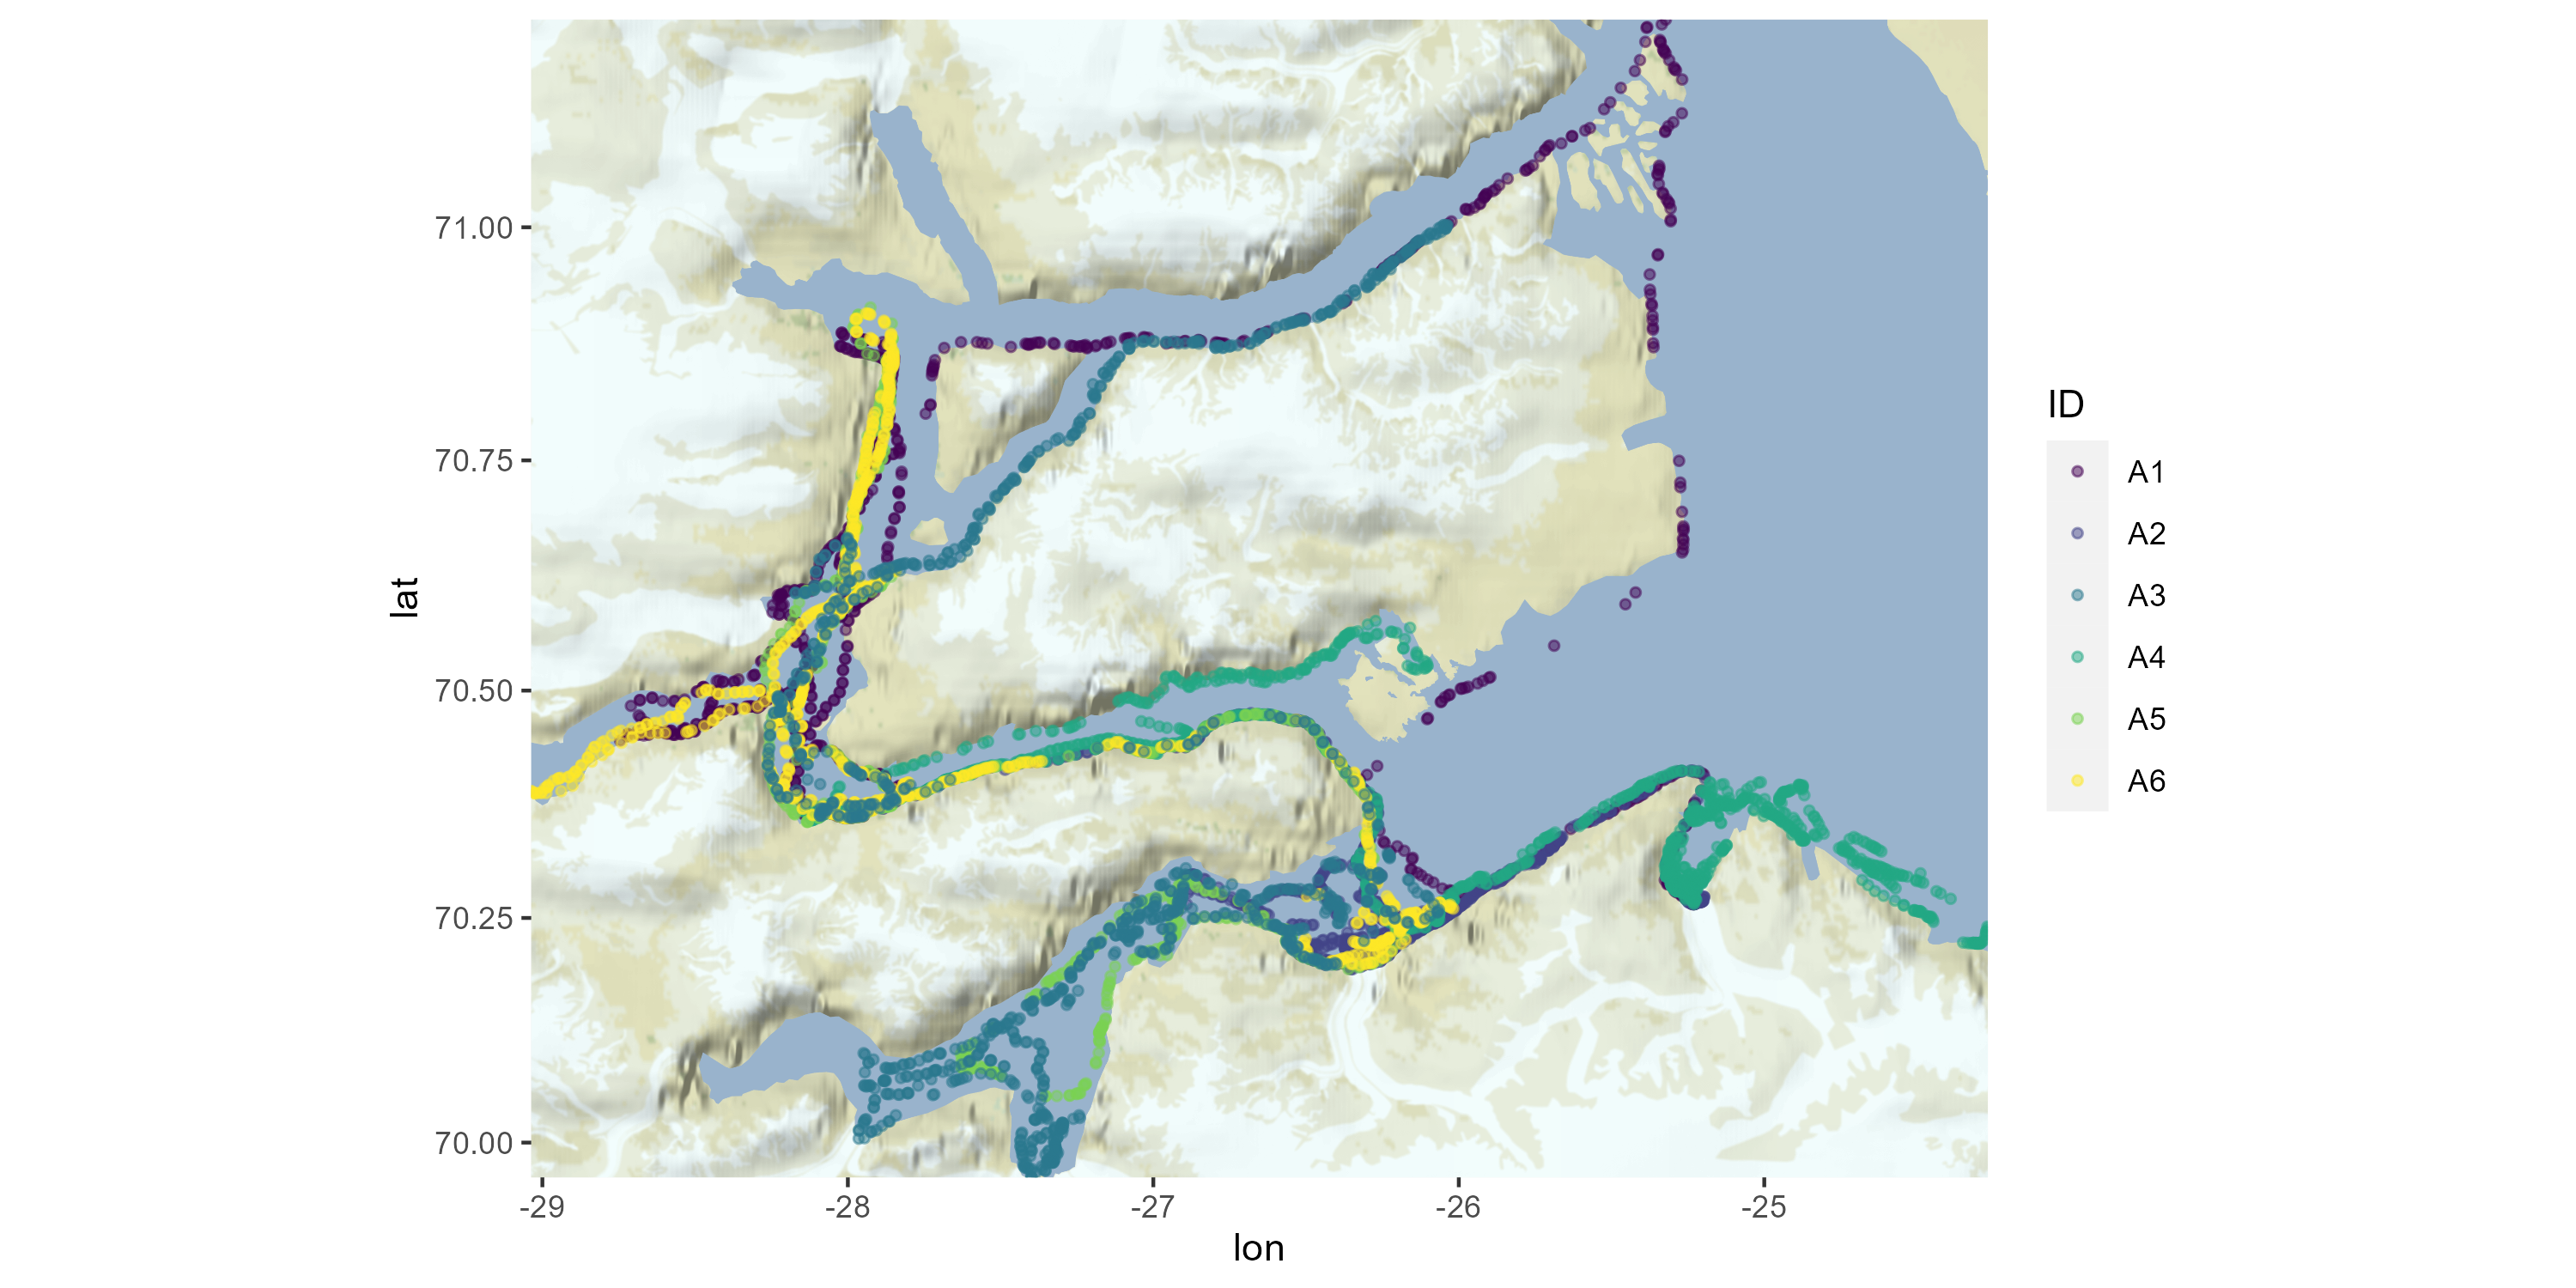
\includegraphics[scale=0.6]{images/data_exploration/all_narwhals_tracks.pdf}
\caption{Observed narwhals GPS tracks. Red crosses indicate the starting points of the trajectories.}
\label{fig: observed GPS data}
\end{figure}


For each narwhal, the entire track is split into two periods: a period before exposure defined as the period before the narwhal gets in line of sight with the ship for the first time, and the period of exposure starting after exposure onset. We discard the GPS measurements from the first 12 hours after tagging, to avoid any tagging effects on the behavior. We applied a velocity filter to keep only positions that have empirical velocity lower than 20 km/h. Two data points were removed with this filter.
Overall, $4815$ GPS positions are kept for the analysis. The splitting between data before and after exposure results in $1558$ measurements before exposure and $3257$ measurements after exposure.

\subsection{Notations and covariates}
\label{subsection: covariates}

For each narwhal $i \in \{1,\ldots,N\}$ with $N=6$, we denote $n_i$ the total number of observations,   decomposed as $n_i=n_{i,pre}+n_{i,post}$ where $n_{i,pre}$ is the number of observations before exposure, and $n_{i,post}$ is the number of observations after exposure onset. The positions are observed at discrete times $t_{i1}, t_{i2}, \cdots,t_{in_i}$ and  for $j \in \{1,\cdots,n_i\}$, we denote $y_{ij}=\begin{pmatrix} y_{ij1} & y_{ij2} \end{pmatrix}^\top$ the observed GPS position at time $t_{ij}$, projected in UTM zone 26 North coordinates with the \texttt{R} package \texttt{rgdal}. These points are noisy observations of the underlying unobserved true positions.\\

The land polygons define the boundaries of the domain $\mathcal{D}$ in which the narwhals can move. It is critical to accurately represent the shoreline geometry to ensure realistic movement constraints within the fjord system. Initially, we used land polygons obtained from OpenStreetMap, but these led to approximately $9\%$ of recorded narwhal positions being incorrectly classified as on land, likely due to inaccuracies in the shoreline representation. To address this, we manually refined the polygons using satellite raster data in QGIS, improving accuracy but still observing some positions classified as on land or unrealistically close to the shoreline (<10 m). To account for both shoreline inaccuracies and potential GPS error, we applied a geometric buffer using the \texttt{st\_buffer} function in \texttt{R} to shrink the land polygons by 200 m. This adjustment significantly reduced the proportion of positions classified as on land to $0.12\%$ and yielded results more consistent with expected narwhal behavior. The shapefile defining the shoreline is made available in Supplementary materials. For each narwhal $i \in\{1, \ldots N\}$ and each time $j\in\{1, \ldots, n_i\}$, the closest point on the shoreline to the observed GPS position $y_{ij}$  is denoted $p_{ij}$. Due to GPS measurement errors, the distance $D^{shore}_{ij}=d(y_{ij},p_{ij})$ is an approximation of the actual distance to the boundary. Distance to shore values range from $0$ to $7.6$ km.
The angle $\Theta_{ij}$ between the narwhal's heading and the shoreline is defined as the angle between the observed empirical velocity $\hat{v}_{ij}=\frac{y_{ij+1}-y_{ij}}{\Delta_{ij}}$, where $\Delta_{ij}=t_{ij+1}-t_{ij}$, and the vector $\vec{n}_{ij}=y_{ij}-p_{ij}$, as illustrated in Figure~\ref{fig: illustration nearest shore points}. A value $\Theta_{ij}=\pm \frac{\pi}{2}$ indicates a movement parallel to the shore, while $\Theta_{ij} \in \left]\frac{\pi}{2},\pi\right] \cup \left]-\pi,-\frac{\pi}{2}\right[$ indicates movement towards the shore. 


\begin{figure}[ht!]
	\centering
	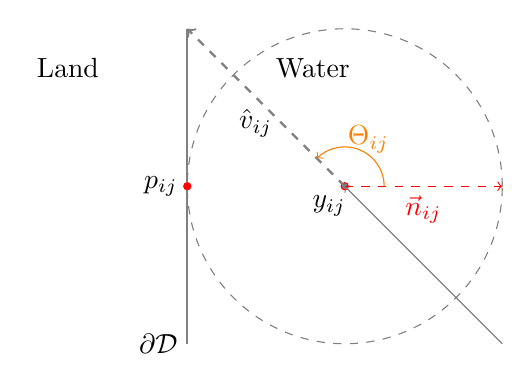
\begin{tikzpicture}
		%boundary
		\draw[gray, thick] (0,0) -- (0,4);
		%position
		\draw[red,fill=gray] (2,2) circle (.3ex);
		%nearest shore point
		\draw[red,fill=red] (0,2) circle (.3ex);
		%velocity
		\draw[->,gray] (4,0) -- (2,2);
		\draw[->,gray,dashed,thick] (2,2) coordinate (O) -- (0,4) coordinate (A);
		%normal vector
		\draw[->,red,dashed] (O) -- (4,2) coordinate (B);
		%trigonometric circle
		\draw[gray,dashed] (2,2) circle (2cm);
		%angle 
		\pic[draw=orange,->,angle eccentricity=1.2,angle radius=0.5cm] {angle=B--O--A};
		
		%nodes
		\node[left] at (-1,3.5) {Land};
		\node[right] at (1,3.5) {Water};
		\node[left] at (0,0) {$\partial \mathcal{D}$};
		\node[left] at (0,2) {$p_{ij}$};
		\node[left] at (1.2,2.8) {$\hat{v}_{ij}$};
		\node[below] at (1.8,2) {$y_{ij}$};
		\node[below,red] at (3,2) {$\vec{n}_{ij}$};
		\node[above,orange] at (2.3,2.3) {$\Theta_{ij}$};
	\end{tikzpicture}
	\caption{Example of nearest point on the shore and angle $\Theta$. $\partial D$ represents the boundary of the domain, $y_{ij}$ is the observed GPS position of narwhal $i$ at time $t_{ij}$.}
	\label{fig: illustration nearest shore points}
\end{figure}

The distance to the ship $D^{ship}$ (km) is defined as the distance between observed GPS locations of the ship and the narwhal. The values are comprised between $2.68$ and $63.8$ km.
Exposure to the ship for narwhal $i$ at time $t_{ij}$, denoted $E^{ship}_{ij}$, is defined as the inverse of the distance to the ship (in km). The covariate $E^{ship}$ is meant to be a proxy for sound exposure levels received by the narwhals. Reasonably, the closer the narwhal is to the ship, the louder is the sound, and thus the exposure is larger. 
$D^{ship}$ is only defined when the narwhal is in line of sight with the ship and exposures are set to $0$ when this is not this case. This implies that in the statistical model, the ship noise is only allowed to affect the narwhal when the ship is in line of sight, though it is likely that narwhals can perceive the disturbance even when they are not in line of sight with the sound source. This provides a conservative estimate of the effect of the noise exposure. Levels of the covariate $E^{ship}$ for each narwhal is displayed in Figure~\ref{fig: realexpthroughtime}.




\begin{figure}[ht!]
		\centering
		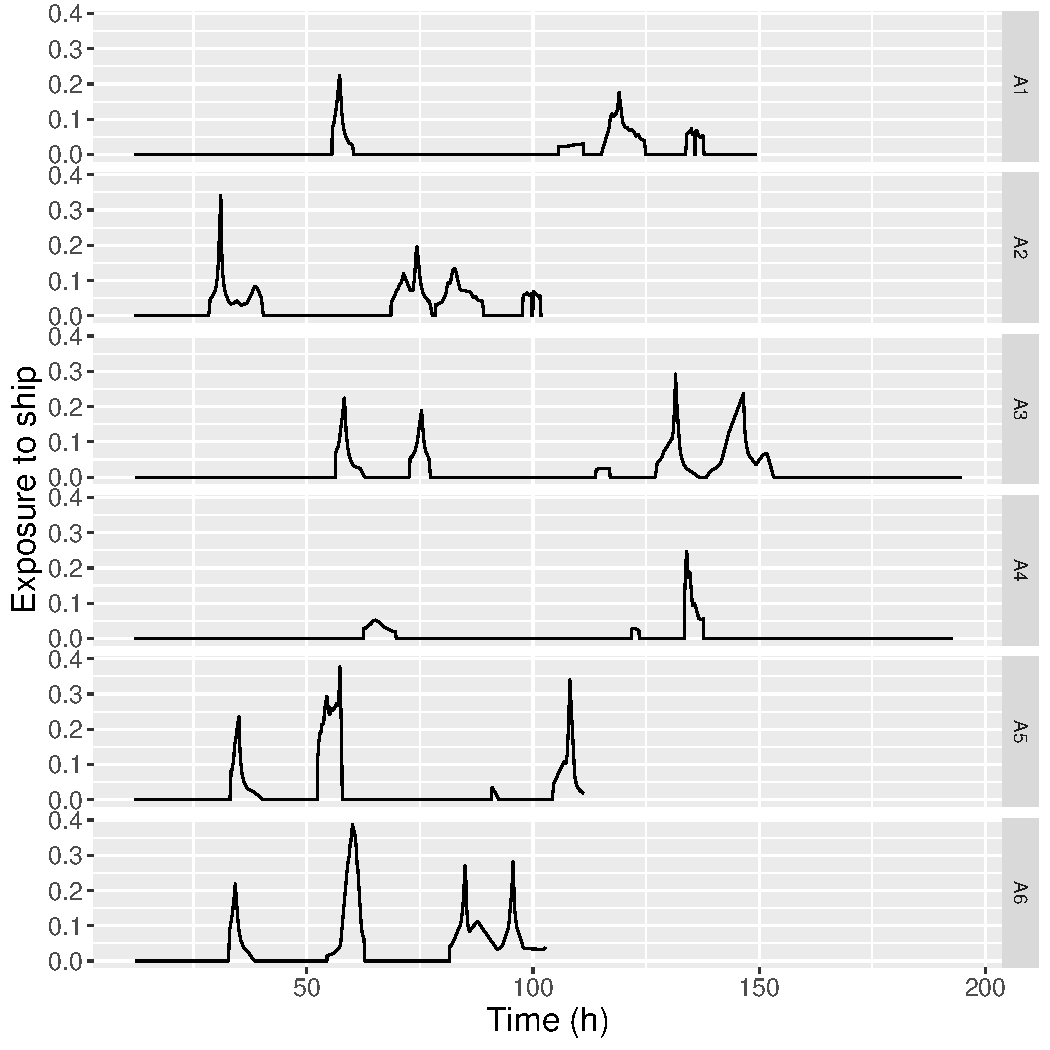
\includegraphics[scale=0.50]{images/data_exploration/realExpShip_through_time.pdf}
	
	\caption{Covariate $E^{ship}$ (in $km^{-1}$) over time for each narwhal. Time 0 corresponds to 12 hours after tagging for each individual whale.}  
	\label{fig: realexpthroughtime}
\end{figure}



\section{Movement models within a constrained landscape}

The dynamics of the true positions of the narwhals is modelled by a SDE. First, we recall the standard rotational CVM \citep{gurarie_correlated_2017}, and then we extend it to include the effect of the distance to shore on the movement and constrain the position within a polygon.


\subsection{Standard Rotational Advective correlated velocity model (RACVM)}
\label{section: RACVM}
\mbox{}\\

Let $A=\begin{pmatrix} 
	\frac{1}{\tau} &&-\omega \\
	\omega && \frac{1}{\tau}
\end{pmatrix}$ and define

\begin{equation} \left\{
	\begin{array}{l}
		dX(t)=V(t)dt \\
		dV(t)=-A(V(t)-\mu)dt+\frac{2\nu}{\sqrt{\pi \tau}} dW(t) 
	\end{array}
	\right.
	\label{eq: RACVM equation}
\end{equation}
where $V(t)$ is the horizontal two-dimensional velocity at time $t$, $X(t)$ is the two-dimensional horizontal position, typically in longitude and latitude or in UTM coordinates, $W(t)$ is a two-dimensional brownian motion. Parameter $\tau$ is an autocorrelation time scale, $\nu$ controls the norm of the velocity and drives the random variability, $\mu=\begin{pmatrix} \mu_1 && \mu_2 \end{pmatrix}^\top$ is the long term velocity, and $\omega$ is an angular velocity that controls how fast the velocity vector rotates. The case $\omega=0$ corresponds to a standard CVM. In most applications, this standard model is satisfactory, but in case of tortuous movement, a non-zero value of $\omega$ is sometimes needed \citep{gurarie_correlated_2017,alt_correlation_1990,albertsen_generalizing_2018}. We will later model $\omega$ as varying over time as a function of the distance to shore and the angle $\Theta$. Whether or not to include a non-zero mean velocity parameter $\mu$ depends on the specific context of the study. Typically, it makes sense to have $\mu\neq (0,0)$ when examining migratory patterns or avoidance reactions from a fixed sound source. We will later consider $\mu=0$ in our model.\\

In this section, we derive the explicit transition density for the process $U=\begin{pmatrix} X && V \end{pmatrix}^\top$. Though this model is considered in several papers, we found no mention of the closed form formulas derived here. In \cite{gurarie_correlated_2017}, only the process $V$ is exhaustively studied, and the classical distributional results about this process are used for estimation and simulation purposes.
A more general formulation is considered by \cite{albertsen_generalizing_2018} in which the diffusion matrix is lower triangular with positive diagonal elements and two distinct autocorrelation parameters are considered in each direction allowing for anisotropic movement. In this case, \cite{albertsen_generalizing_2018} derives the Gaussian transition density of the velocity process, where the covariance matrix is expressed using a Kronecker sum. However, the formulas for the process $X$
are not provided, and the Euler scheme is employed to approximate the transition densities of $X$. This approach is generally sufficient when the animal’s positions are recorded at high frequency. Yet, for marine mammals such as narwhals that dive to great depths, GPS measurements are usually taken at irregular intervals, typically of several minutes, which can render the Euler scheme unsuitable. Additionally, incorporating covariates into the parameters of the SDE often requires approximating the transition density by assuming the covariates remain constant during each time step \citep{michelot_varying-coefficient_2021}. This results in two layers of approximation, possibly leading to unreliable estimation.\\

Here, we derive a closed form formula for the transition density of the Markov process $(X ,V)$ under the hypothesis of isotropic movement, with diagonal diffusion matrix as in~\eqref{eq: RACVM equation}.\\


\begin{proposition}
	Let $U(t)=\begin{pmatrix} X(t) && V(t) \end{pmatrix}^\top$ for $t \geq 0$ be the solution to \eqref{eq: RACVM equation}. Then the exact transition density of the Markov process $U$ is given by 
	\begin{equation}
		U(t+\Delta) \vert U(t)=u \sim \mathcal{N}\left( T(\Delta) u +B(\Delta)\mu, Q(\Delta)\right) \mbox{ for all } \Delta>0 \mbox{ and } u \in \R^4
		\label{eq: X V distribution}
	\end{equation}
	where \begin{equation}
		T(\Delta)=\begin{pmatrix} I_2 && A^{-1}(I_2-\exp(-A\Delta)) \\
			0_2 && \exp(-A\Delta) \end{pmatrix} \mbox{, } B(\Delta)=\begin{pmatrix}
			\Delta I_2 -A^{-1}(I_2-\exp(-A\Delta))\\
			I_2-\exp(-A\Delta)\end{pmatrix}
		\label{eq: link matrices}
	\end{equation}
	and the covariance block matrix is given by
	\begin{equation}
		Q(\Delta)=\begin{pmatrix}
			q_1(\Delta)I_2 && \Gamma(\Delta) \\
			\Gamma(\Delta)^\top && q_2(\Delta)I_2
		\end{pmatrix}
		\label{eq: covariance matrix}
	\end{equation}
	with 
	\begin{equation*}q_1(\Delta)=\frac{\sigma^2}{C}\left( \Delta-2 \frac{\omega \sin(\omega \Delta)-\frac{1}{\tau} \cos(\omega \Delta)}{C} \exp\left( -\frac{\Delta}{\tau} \right) +\frac{\tau}{2} \left( \frac{\omega^2-\frac{3}{\tau^2}}{C}-\exp\left( -\frac{2\Delta}{\tau}\right)\right) \right)
	\end{equation*}
	
	\begin{equation*}
		q_2(\Delta)=\frac{2\nu^2}{\pi}\left(1-e^{-\frac{2 \Delta}{\tau}}\right)
	\end{equation*}
	\begin{equation*}\Gamma(\Delta)=\begin{pmatrix} \gamma_1 && \gamma_2 \\
			-\gamma_2 && \gamma_1\end{pmatrix}
	\end{equation*}
	where
	\begin{equation*}\gamma_1=\frac{\sigma^2}{2 C } \times \left( 1+\exp\left( -\frac{2\Delta}{\tau}\right)-2\exp\left( -\frac{\Delta}{\tau}\right) \cos(\omega\Delta)\right)
	\end{equation*}
	\begin{equation*}\gamma_2=\frac{\sigma^2}{C} \times\left( \exp\left( -\frac{\Delta}{\tau}\right) \sin(\omega \Delta)-\frac{\omega \tau}{2} \left(1-\exp\left( -2 \frac{\Delta}{\tau}\right) \right)\right)
	\end{equation*}
	and we denoted $C=\frac{1}{\tau^2}+\omega^2$ and $\sigma=\frac{2\nu}{\sqrt{\pi \tau}}$.
	\label{prop: transition density}
\end{proposition}

The formulas derived in \citep{johnson_continuous_2008} are a corollary of Proposition~\ref{prop: transition density}, obtained with $\omega=0$. The proof of this proposition is detailed in Appendix.

Equation~\eqref{eq: covariance matrix} shows that the two components of the location and velocity processes are independent.
Note that $\exp(-A\Delta)=e^{\frac{-\Delta}{\tau}} \begin{pmatrix} \cos(\omega \Delta) && \sin(\omega \Delta) \\ -\sin(\omega \Delta) && \cos(\omega \Delta) \end{pmatrix}$ is a weighted rotation matrix of angle $-\omega \Delta$.
Intuitively, ~\eqref{eq: X V distribution} means that the next velocity $V(t+\Delta)$ is a weighted mean of the long term mean velocity $\mu$ and the previous velocity $V(t)$ rotated by an angle $-\omega \Delta$.\\


For locomotion under spatial constraints, we hypothesize that an increase in tortuosity is a sign of avoiding the boundary and adapting the heading to the spatial constraint. We use this to define a constrained version of the standard RCVM.

\subsection{Constrained rotational correlated velocity model}
\label{section: CRCVM}

We propose a new RCVM that relies on the tortuosity parameter, or angular velocity $\omega$, to describe how the animals turn in reaction to the shore. 
To do so, we consider $\omega$ as a smooth function both of the distance to the shore $D^{shore}$ and the angle between the velocity vector and the shore normal vector $\Theta$. 
We write $\mathcal{D} \subset \R^2$ for the polygon defining the domain of the process $X$. The new formulation of the equation is 
\begin{equation} \left\{
	\begin{array}{l}
		dX(t)=V(t) dt \\
		dV(t)=-A(X(t),V(t))V(t)dt+\frac{2\nu}{\sqrt{\pi \tau}} dW(t) 
		
	\end{array}
	\right.
	\label{eq: CRCVM equation}
\end{equation}
with 
\begin{equation} 
	A(X(t),V(t))=\begin{pmatrix} 
		\frac{1}{\tau} && -\omega(X(t),V(t)) \\
		\omega(X(t),V(t)) && \frac{1}{\tau}
	\end{pmatrix}
	\label{eq: CRCVM matrix A}
\end{equation}
where $\omega(X(t),V(t))=f(D^{shore}(t),\Theta(t))$ with  $f_{\omega}$ a smooth function from $\R^{+} \times ]-\pi,\pi]$ to $\R$. In the sequel, such models will be refered to as Constrained Rotational Correlated Velocity Models (CRCVM).\\

To induce a rotation when the animal is close to the boundary and heading in the direction of the shore,
the following assumptions must guide the shape of $f$:
\begin{itemize}
	\item[1)] for a distance to the shore lower than some threshold, $f(D^{shore},\cdot)$ should be positive and increasing on $]\frac{\pi}{2},\pi]$, 
	\item[2)] for a distance to shore  lower than some threshold, $f(D^{shore},\cdot)$ should be negative and decreasing on $]-\pi,-\frac{\pi}{2}[$,
	\item[3)] as distance to shore decreases, the magnitude of the functions  $f(D^{shore},\cdot)$ on $]\frac{\pi}{2},\pi[$  and $]-\pi,-\frac{\pi}{2}[$ should increase.
\end{itemize} 


We propose a parametric model for the function $f$. For $\Theta \in ]-\pi,\pi]$ and $D^{shore} \geq 0$, we define $f$ as the sum of a repulsive term and an attractive term :

\begin{equation}
	\label{eq: smooth omega}
	f(\Theta,D^{shore})=g(\Theta,D^{shore})+h(\Theta,D^{shore}))
\end{equation}
where 
\[g(\Theta,D^{shore})=a\theta\left(\theta-\frac{\pi}{2}\right)\left(\theta+\frac{\pi}{2}\right)\times \frac{1}{D_{shore}}\exp\left(-\frac{D_{shore}}{D_0}\right)\]is the repulsive term and \[h(\Theta,D^{shore})=b\exp\left(-\left(\begin{pmatrix} \Theta & D^{shore} \end{pmatrix}-m\right) \Sigma^{-1} \left(\begin{pmatrix} \Theta & D^{shore}\end{pmatrix}-m)^\top \right)\right)\]
is the attractive term. Here, $ m=(\frac{\pi}{2\sqrt{3}},D_1)$, $\Sigma=\begin{pmatrix} \sigma_D^2 & 0 \\ 0 & \sigma_\Theta^2\end{pmatrix}$ and $D_a,D_b>0$, $a,b>0$ , $\sigma_D,\sigma_\Theta >0$ are parameters.
The parameter $a$ controls the magnitude of the angular velocity, $D_a$ controls the distance at which the velocity starts to rotate to model repulsion from the boundary and $D_b$ controls the distance at which the velocity starts to rotate to model attraction to the boundary. Then, $ \sigma_D$ and $\sigma_\theta$ are the standard deviations in the gaussian kernels. Figure~\ref{fig: perspectiveplots}  shows function~\eqref{eq: smooth omega}.

\begin{figure}[ht!]
	\centering
		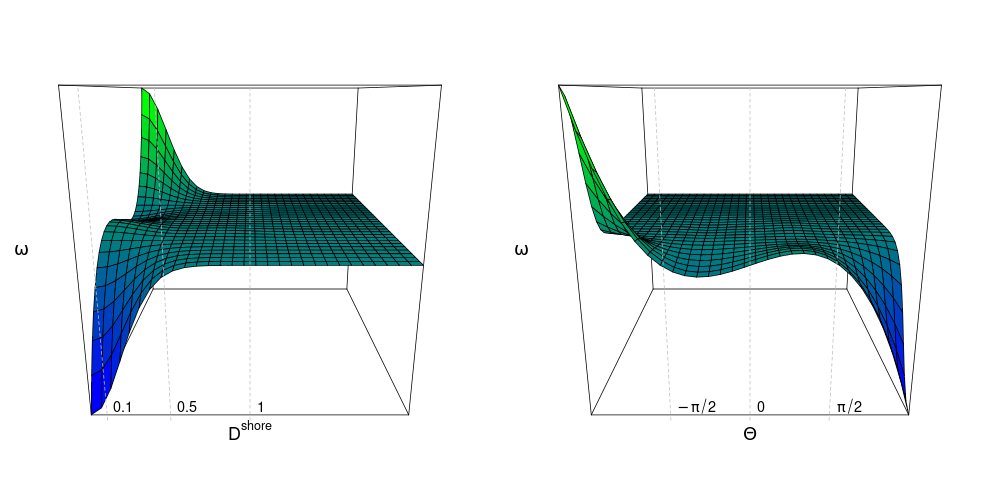
\includegraphics[scale=0.4]{images/crcvm/perspective_plots.png}
		

\caption{Example of smooth functions $f_{\omega}$ defined by~\eqref{eq: smooth omega}. Angular velocity $\omega$ increases in absolute value as $\Theta$ approaches $\pm\pi$, and decreases with increasing distance to the shore.  Here, angle $\Theta$ is in $rad$ and $D^{shore}$ in $km$. Parameter values are $a=1$, $b=5$, $D_0=0.3$ km,$D_1=0.8$ km, $\sigma_{\theta}=\pi/8$ rad , $\sigma_D=0.2$ km.}
\label{fig: perspectiveplots}
	
\end{figure}


Compared to the reflected CVM in \cite{hanks_reflected_2017}, model~\eqref{eq: CRCVM equation} is very flexible, and different species-specific behaviours can be described. The function $f$ controls at which distance the animal will turn away from the shore, and how fast it will turn.  Specific constraints on $f$ can be set from biological knowledge about the species in question. 

Solving explicitly~\eqref{eq: CRCVM equation} is out of reach due to the non-linearity induced by the distance to the shore and the angle $\Theta$. But it is possible to get an approximate solution. We choose a small time step $\Delta$ and approximate $D^{shore}$ and $\Theta$ by piecewise constant functions on each time step. We then use the formulas of Section~\ref{section: RACVM} to simulate the process and get the next position from the approximate transition densities. Simulated trajectories obtained within the fjords domain are shown in Figure~\ref{fig: crcvm examples} and compared to trajectories simulated from a reflected CVM \citep{hanks_reflected_2017}. Trajectories of our model are effectively constrained and show different features from the reflected CVM : movement along and close to the boundary is favoured.   \\

\begin{figure}[ht!]
	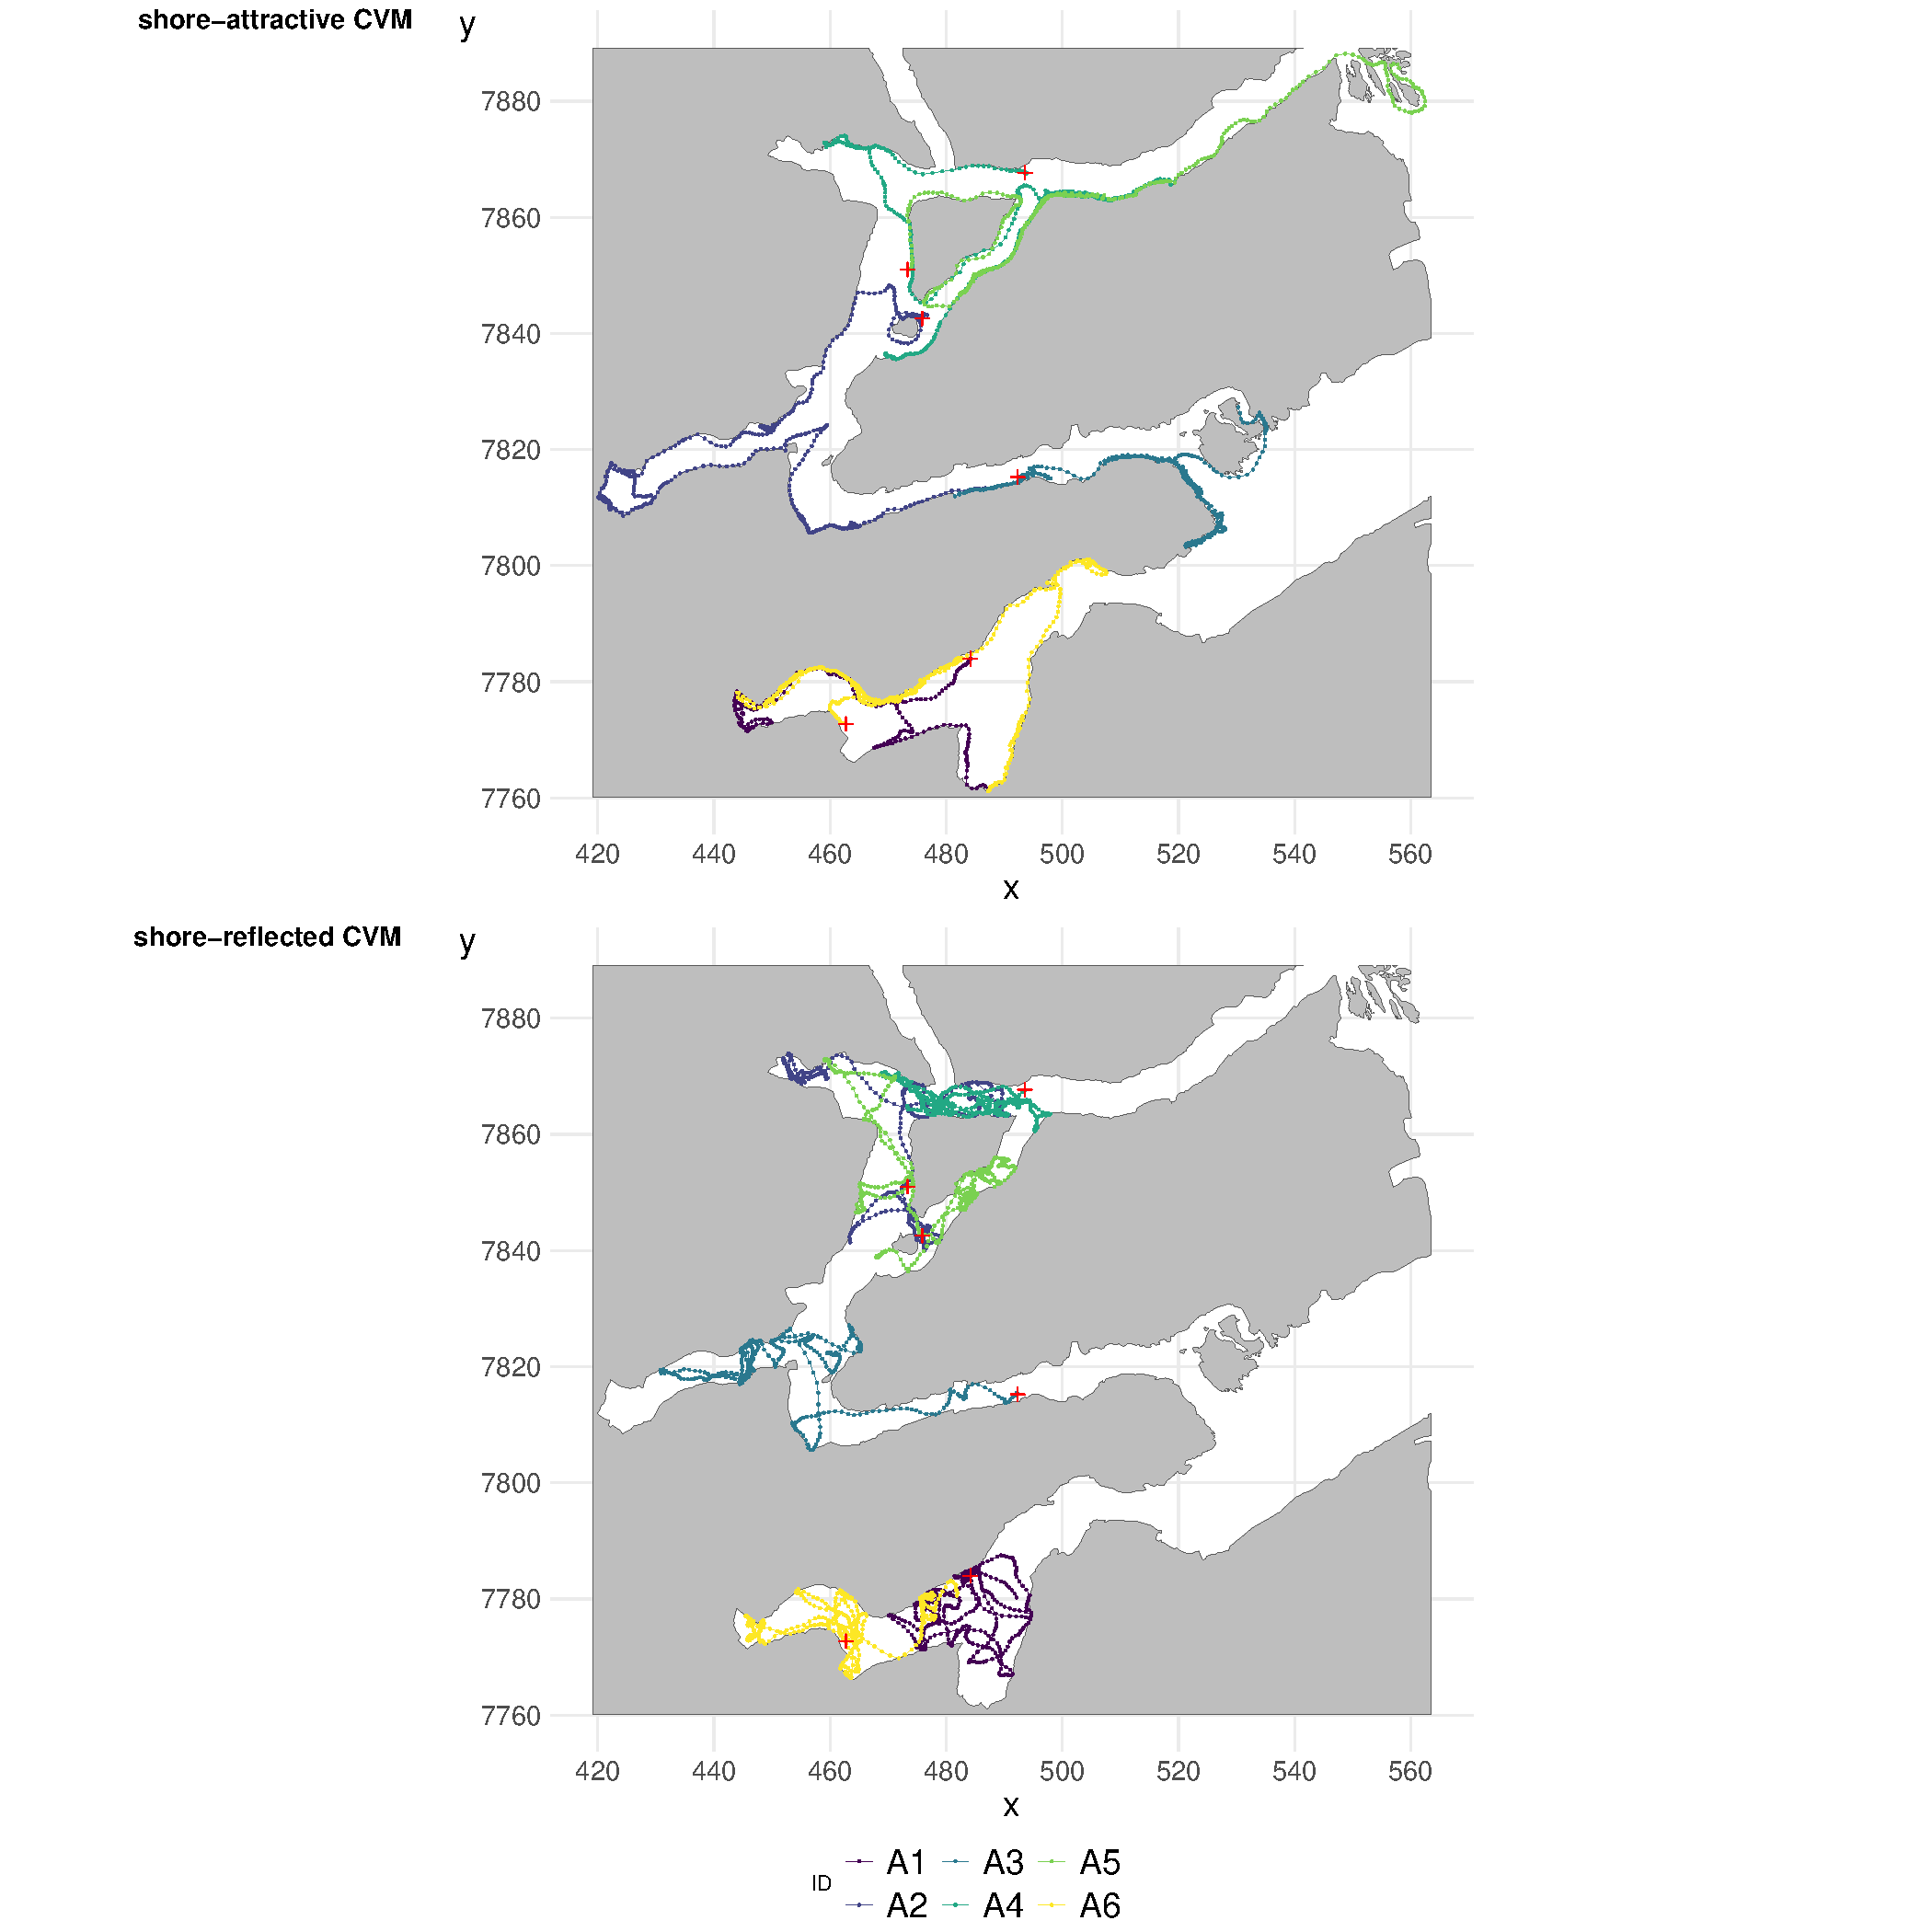
\includegraphics[scale=0.42]{images/crcvm/illustrative_trajectories_fjords.pdf}

	\caption{Three days long simulated trajectories for $6$ different initial positions within the fjords domain for the CRCVM defined by equation~\eqref{eq: CRCVM equation} (top) and the reflected CVM in \cite{hanks_reflected_2017} (bottom). Trajectories are simulated with fixed time step $\Delta= 10 $s and then subsampled to $10 $ min. All trajectories have constant velocity parameter $\nu=4$ km/h and constant persistence $\tau=2$ h.}
 \label{fig: crcvm examples}
\end{figure}



While we have not established formal theoretical conditions for the function $f_{\omega}$ to guarantee constrained motion,  illustrative examples demonstrate how smooth, interpretable functions can produce constrained trajectories for the process $X$. A critical parameter in this model is the spatial scale of the rotational movement, defined as $\rho=\frac{\nu}{\vert \omega \vert}$, representing the diameter of rotation. We hint that $\rho$ should remain smaller than $D^{shore}$ in order to reduce the probability of the process hitting the boundary, .\\


We will use the CRCVM \eqref{eq: CRCVM equation} allowing $\omega$ to vary to analyze narwhals trajectories while considering spatial constraints, whereas we keep $\tau$ and $\nu$ fixed. We detail the statistical model in the next section.






\section{Inference of the sound exposure effect}

To analyse potential perturbations in the locomotion of the narwhals due to sound exposure, we formulate a statistical mixed effect model for the parameters of the CRCVM, and discretise~\eqref{eq: X V distribution} to get an approximate state space model for inference with the Kalman filter.


\subsection{Mixed effect CRCVM for  shore influence and sound exposure}
\label{subsection: ship exposure effect}


First a baseline model is fitted only on the data before exposure, to get an estimate of natural behavior, when the narwhals are not exposed to the ship and airgun sounds. Then, a response model is fitted on the data during exposure to test whether the estimated smooth parameters deviate significantly from the baseline values. We present here the baseline and response models.\\

For the baseline model, only the effect of the shore is included through the covariates $D^{shore}$ and $\Theta$. For each narwhal $i \in \{1, \cdots, N\}$ and each time $j\in\{1, \cdots, n_{i,pre}\}$, $y_{ij}$ is an observation with measurement error of position $X_{ij}$:

\begin{equation}
	y_{ij}=X_{ij}+\varepsilon_{ij} \quad 
	\varepsilon_{ij} \underset{i.i.d}{\sim} \mathcal{N}(0,\sigma_{obs}^2)  
	\label{eq: baseline observations}
\end{equation}

The standard deviation $\sigma_{obs}$ represents GPS measurement errors variability. The assumption of i.i.d. Gaussian measurement errors is a simplified model of actual GPS measurement errors. In practice, the accuracy of GPS positions is influenced by the number of satellites processing the GPS signal—more satellites generally result in more accurate positions. Furthermore, the error can differ between the $x$ and $y$ directions. For a comprehensive study on Fastloc-GPS measurement errors, we refer to \cite{wensveen_path_2015}. It is often more appropriate to use a distribution with heavier tails, such as the Student's $t$-distribution, to model measurement error. However, this introduces additional complexity to the inference process, as a standard linear Kalman filter introduced by \cite{johnson_continuous_2008}
cannot be directly applied in such cases. Since the Student's $t$-distribution approaches a Gaussian distribution as its degrees of freedom increase, the Gaussian distribution is considered a reasonable trade-off between simplicity and suitability.\\

%We denote $\tau_i$, $\nu_i$, $\omega_i$ the parameters of the CRCVM for narwhal $i$. 
The latent processes $X_i$ and $V_i$ are solutions do


\begin{equation}  %\forall i \in \{1,\cdots,N\}, \quad 
	\left\{
	\begin{array}{l}
		dX_i(t)=V_i(t)dt  \\
		dV_i(t)=-\begin{pmatrix} 
			\frac{1}{\tau_i} && -\omega_i(t) \\
			\omega_i(t) && \frac{1}{\tau_i}
		\end{pmatrix}V_i(t)dt+\frac{2\nu_i}{\sqrt{\pi \tau_i}} dW(t) \\
	\end{array}
	\right.
	\label{eq:baseline latent processes}
\end{equation}
%
where $\tau_i$, $\nu_i$ are individual parameters   to account for variability between narwhals:
%
\begin{equation}   
	%\begin{array}{l}
	\begin{pmatrix}	\log(\tau_i)\\ \log(\nu_i) \end{pmatrix}
	= \begin{pmatrix}\log(\tau_0)\\ \log(\nu_0) \end{pmatrix}
	+
	\begin{pmatrix} b_{\tau,i}\\  b_{\nu,i}  \end{pmatrix}
	\quad \mbox{ with } \quad
	\begin{pmatrix} b_{\tau,i} \\ b_{\nu,i} \end{pmatrix} \underset{i.i.d}{\sim} \mathcal{N}\left(0,\begin{pmatrix} \sigma_{\tau}^2 && 0 \\ 0 && \sigma_{\nu}^2 \end{pmatrix}\right) 
	%\end{array}
	\label{eq:baseline random effects}
\end{equation}

Since $\tau$ and $\nu$ are positive, a log link function is used for these parameters. The coefficients $\log(\tau_{0})$, $\log(\nu_{0})$ are population intercepts and $b_{\tau,i}$, $b_{\nu,i}$
are the individual random effects. \\

Finally, as discussed in Section \ref{section: CRCVM}, the angular velocity $\omega_i$ for individual $i$ is expressed as a smooth function of $\Theta$ and $D^{shore}$ : 
%
\begin{equation} 
	\omega_i(t)=f(D^{shore}(t),\Theta(t);a,b,D_a,D_b,\sigma_D,\sigma_\Theta)
\end{equation}
where the function $f$ is defined in equation \eqref{eq: smooth omega}. The parameters $a$,$b$,$D_a$,$D_b$, $\sigma_D$ and $\sigma_\Theta$ will be considered as fixed and known.
\\

The response model is then designed to assess a deviation from the baseline model due to exposure to the ship. The observations are supposed to have the same measurement errors as the baseline. For $i \in \{1, \ldots, N\}$ and $j \in \{n_{i,pre}+1,\cdots,n_{i,post}\}$, we have

\begin{equation}  		y_{ij}=X_{ij}+\varepsilon_{ij}, \quad 		\varepsilon_{ij} \underset{i.i.d}{\sim} \mathcal{N}(0,\sigma_{obs}^2) 
	\label{eq: response observations}
\end{equation}

Then we add a dependency on the covariate $E_{ship}$ in the parameters $\tau_i$ and $\nu_i$: 
\begin{equation}    
	\begin{array}{l}
		\log(\tau_{i}(t))=\log(\tau_{0})+\alpha_{\tau} E^{ship}_i(t)+b_{\tau,i} \\
		\log(\nu_{i}(t))=\log(\nu_{0}) +  \alpha_{\nu} E^{ship}_i(t) +b_{\nu,i}  \\
	\end{array}
	\label{eq:response loglinear model}
\end{equation}


The intercepts $\log(\tau_0)$, $\log(\nu_0)$ and the smooth $\omega$ from the baseline model enter as offsets in the response model.
Thus, only the coefficients $\alpha_{\tau}$ and $\alpha_{\nu}$ are estimated from the data during exposure. These parameters control the deviation of $\tau_i$ and $\nu_i$ from their baseline values $\tau_0$ and $\nu_0$ as a function of the distance to the ship. Coefficients $\alpha_{\tau}$ and $\alpha_{\nu}$ significantly deviating from $0$ indicate an effect of the sound exposure on the narwhals horizontal motion.




\subsection{Approximate linear Gaussian state-space model}
\label{section: state space model}

In the baseline statistical model \eqref{eq:baseline latent processes}, we make the approximation suggested in \citep{michelot_varying-coefficient_2021} that the time-varying parameter $\omega_i$ is piecewise constant.
On each time step $[t_{ij},t_{i,j}+\Delta_{ij}]$ between two observations, we interpolate valus of $D^{shore}_i$ and $\Theta_i$ at times $t_{ij}^{(0)} = t_{ij} < t_{ij}^{(1)} < \cdots < t_{ij}^{(k)}=t_{ij}+\Delta_{ij}$ by fitting splines on the observed trajectories.

We write $U_{ij}=\begin{pmatrix} X_{ij,1}  && X_{ij,2} && V_{ij,1} && V_{ij,2}\end{pmatrix}^\top$ and for $l \in \{0,\cdots,k\}$,
\[\omega_{ij}^{(l)}=\omega(t_{ij}^{(l)}), \quad   A_{ij}^{(l)}=\begin{pmatrix} 
	\frac{1}{\tau_{i}} && -\omega_{ij}^{(l)} \\
	\omega_{ij}^{(l)} && \frac{1}{\tau_{i}}
\end{pmatrix} \]


We use the formulas from Proposition \ref{prop: transition density} to obtain an approximation of the state-space matrix equations for each individual $i\in\{1,\ldots, N\}$, and each observation $j\in\{1, \ldots, n_{i,pre}\}$ when $\omega$ varies with time. We write $T_{ij}^{(l)}=T(\Delta_{ij}^{(l)})$ and $Q_{ij}^{(l)}=Q(\Delta_{ij}^{(l)})$ as defined in \eqref{eq: link matrices} and \eqref{eq: covariance matrix}.
Then the approximate transition density is 
	\begin{equation}
	U_{i,j+1} \vert U_{ij}=u \sim \mathcal{N}\left( \tilde{T}_k(\Delta_{ij}) u, \tilde{Q}_k(\Delta_{ij})\right)
	\label{eq: approximate transition density}
\end{equation}
where 
    \begin{equation}
    \tilde{T}_k(\Delta) = T_{k-1} \times \cdots \times T_1 \times T_0 
    \end{equation}
and 
    \begin{equation}
        \tilde{Q}_k(\Delta) =\sum_{l=1}^{k} T_{k-1}^\top \cdots T_{l+1}^\top Q_l T_{l+1} \cdots T_{k-1}
    \end{equation}

Thus we obtain the following approximate linear state-space model 
\begin{equation}
	\begin{array}{l}
		y_{ij}=ZU_{ij}+\varepsilon_{ij},  \quad 
		\varepsilon_{ij} \underset{i.i.d}{\sim} \mathcal{N}(0,\sigma_{obs}^2) \\
		U_{i,j+1}=\tilde{T}_{ij}\,U_{ij} + \eta_{ij}, \quad 
		\eta_{ij} \sim \mathcal{N}(0,\tilde{Q}_{ij})
	\end{array}
	\label{eq: RACVM state space}
\end{equation}
where $Z=\begin{pmatrix} I_2 && 0_{2,2}\end{pmatrix}$, $\tilde{T}_{ij}=\tilde{T}_k(\Delta_{ij})$ and $\tilde{Q}_{ij}=\tilde{Q}_k(\Delta_{ij})$.
\\
An approximate linear Gaussian state-space model is obtained similarly for the response model. Estimation with $\texttt{smoothSDE}$ relies on this state-space formulation.
The complete likelihood is computed from the observations $y_{ij}$ as a by-product of the Kalman filter algorithm \citep{michelot_varying-coefficient_2021}.
Laplace's approximation of the integral of this complete likelihood over the random effects is computed using the \texttt{R} package \texttt{TMB}  and optimization is performed via the \texttt{optim} function in $\texttt{R}$ with the BFGS gradient method, with the gradient being calculated by automatic differenciation. We refer to \citep{kristensen_tmb_2016} for more details about the derivation of the multidimensional Laplace's approximation and the gradient computations.
This method is already implemented for the CVM ($\omega=0$) in \texttt{smoothSDE}. Here, we extend this inference method to the more general model~\eqref{eq: CRCVM equation} and use it for estimation of the baseline and the response models.




\section{Simulation study for the baseline model}
\label{section: simulation constrained motion}
To test the estimator of the constrained model for our application, we simulate CRCVM trajectories over one day in the Scoresby Sound fjord system. We consider observations of a baseline model as described in Section~\ref{subsection: ship exposure effect}. We fix $\tau_0=1.5$ h and $\nu_0=4$ km/h. The random effects standard deviations for the parameters $\tau$ and $\nu$ are set to $\sigma_{\tau}=0.2$ and $\sigma_{\nu}=0.1$. The smooth function $\omega$ is defined as in equation \eqref{eq: smooth omega} with parameter values $D_0=0.5$,$D_1=1$,$a=2$,$b=4$,$\sigma_\theta=\frac{\pi}{8}$, $\sigma_D=0.3$. Initial velocities are set to $(0,0)$ and initial positions are uniformly sampled between $0.1$ and $1$ km from the shore in the fjord system. $1.02\%$ of the simulated trajectories reached land. The batches containing at least one trajectory that reached land were not used for the estimation.\\

Two scenarios are considered: an ideal scenario where we have high frequency data with either high or low measurement error, and a practical scenario where the data is low frequency and measurement errors are high. For each setup, we simulate $M=100$ batches of $N$ individual trajectories with $N \in \{6,12\}$. The time steps between consecutive observations are set $\Delta_{high}=1$ min for high frequency and $\Delta_{low}=5$ min for low frequency. The trajectories are simulated with time step $\Delta =1$ min and then subsampled to $\Delta_{high}$ for low frequency observations. Measurement noise is Gaussian with standard deviation $\sigma_{obs,high}=40$ m and $\sigma_{obs,low}=10$ m for high and low measurement errors. They are supposed to be fixed and known in this simulation study.
  
For the estimation, we fix initial parameter values to $\tau_{0}=1$ h, $\nu_{0} = 1$ km/h, $\sigma_{\tau}=0.5$, $\sigma_{\nu}=0.5$. 
For each batch of $N$ trajectories, we obtain estimates $\widehat{\tau_{0}}^{(k)}$, $\widehat{\nu_{0}}^{(k)}$, $\hat{\sigma}_{\tau}^{(k)}$ and $\hat{\sigma}_{\nu}^{(k)}$, $k \in \{1,\cdots,M\}$ and compute the mean  and the standard error of the estimates. Simulation and optimization of the log-likelihood for one single batch of trajectories in all scenarios are performed on $16$ CPU cores in about $5$ h. Parallelization within \texttt{R} is used to simulate the trajectories, compute the angle $\theta$ and the distance $D^{shore}$, and fit the models in the different scenarios. \\


We estimated all the parameters while considering the smooth function $\omega$ to be known. We used the true $D^{shore}$ and $\theta$, the observed noisy $D^{shore}$ and $\theta$ and smoothed $D^{shore}$ and $\theta$ obtained after fitting splines on the trajectories with \texttt{gam} function in \texttt{R} software. The results are shown in Table~\ref{table: simulation study hf parametric}. This simulation study shows that the main difficulty in the estimation is the parameter $\tau_0$. While we are able to get an unbiaised estimate with the true $D^{shore}$ and $\theta$ from high frequency observations, both the observed and smoothed $D^{shore}$ and $\theta$ yield biaised estimates of $\tau_0$. We also show the estimates obtained for the SDE model with a constant $\omega=0$, which corresponds to the CTCRW in \cite{johnson_continuous_2008}.

	
	\begin{table}[ht!]
		\centering
		\begin{tabular}{|c|c|cccc|}
			\hline
			     & &\multicolumn{2}{|c}{\textbf{Intercepts}}  & \multicolumn{2}{c|}{\textbf{Random effects}} \\
			\cline{3-6}
			     \textbf{Model type} & &$ \tau_0 $ (h) & $\nu_0 $ (km/h)& $\sigma_{\tau}$ & $\sigma_{\nu}$  \\
			\cline{2-6} 
			& True & $1.50$ & $4.00$ & $0.2$ & $0.1$ \\
			\hline
			\multicolumn{6}{|c|}{\textbf{Low measurement error} ($\sigma_{obs} =10$ m)} \\
			\hline
            \multirow{4}{6em}{CTCRW} & \multirow{2}{4em}{$N=6$}  & $1.05$ &
			$4.07$ &
			$0.20$ & $0.08$ 
			\\
			& & $\pm 0.11$ &
			$\pm 0.21$ &
			$\pm 0.11$ & 
			$\pm 0.05$ 
			
			\\
			%\cline{2-6}
			& \multirow{2}{4em}{$N=12$} & $1.04$ &
			$4.07$ &
			$0.23$ & $0.09$ 
			\\
			& & $\pm 0.08$  &
			$ \pm 0.11$ &
			$ \pm 0.10 $ & $ \pm 0.03$ 
            \\
            \hline
			\multirow{4}{6em}{CRCVM \hspace{0.1cm} True} & \multirow{2}{4em}{$N=6$} & $1.42$ &
			$4.09$ &
			$0.23$ &
			$0.12$
			
			\\
			& &	$[1.20,1.74]$ &
			$ [3.77,4.49] $&
			$[0.17,0.28]$ & $ [0.09,0.28]$ 
			\\
            %\cline{2-6} 
			& \multirow{2}{4em}{$N=12$} & $1.48$ &
			$4.03$ & $0.25$ & $0.10$
			
			\\
			& & $[1.29,1.72]$ &
			$  [3.79,4.33]$ &
			$ [0.18,0.30]$ &
			$ [0.08,0.17]$ 
			\\
            \hline
            \multirow{4}{6em}{CRCVM Observed} & \multirow{2}{4em}{$N=6$} & $1.16$ &
			$4.12$ &
			$0.24$ &
			$0.13$
			
			\\
			& &	$[0.93,1.44]$ &
			$[3.76,4.50]$&
			$[0.16,0.36]$ & $[0.07,0.30]$ 
			\\
            %\cline{2-6}
			& \multirow{2}{4em}{$N=12$} & $1.15$ &
			$4.01$ & $0.25$ & $0.10$
			
			\\
			& & $ [1.01,1.30]$ &
			$ [3.75,4.25]$ &
			$[0.17,0.34]$ &
			$[0.07,0.16]$ 
			\\
			\hline	
			\multirow{4}{6em}{CRCVM Smoothed} & \multirow{2}{4em}{$N=6$}  & $1.27$ &
			$4.10 $ &
			$0.24$ & $0.14$ 
			\\
			& & $[1.02,1.51]$ &
			$[3.74,4.47]$ &
			$[0.15,0.36]$ & 
			$[0.08,0.40]$ 
			
			\\
			%\cline{2-6}
			& \multirow{2}{4em}{$N=12$} & $1.29$ &
			$4.03$ &
			$0.28$ & $0.12$ 

			\\
			& & $[1.11,1.42]$  &
			$ [3.85,4.20]$ &
			$ [0.18,0.39]$& $[0.07,0.18] $  \\
            \hline
			\multicolumn{6}{|c|}{\textbf{High measurement error} ($\sigma_{obs} =40$ m)} \\
			\hline
            \multirow{4}{6em}{CTCRW} & \multirow{2}{4em}{$N=6$}  & $1.05$ &
			$4.06$ &
			$0.17$ & $0.09$ 
			\\
			& & $\pm 0.10$ &
			$\pm 0.21$ &
			$\pm 0.13$ & 
			$\pm 0.05$ 
			\\
			%\cline{2-6}
			& \multirow{2}{4em}{$N=12$} & $1.04$ &
			$4.04$ &
			$0.17$ & $0.09$ 
			\\
			& & $\pm 0.07$  &
			$ \pm 0.11$ &
			$ \pm 0.12 $ & $ \pm 0.03$ 
            \\
            \hline
            \multirow{4}{6em}{CRCVM \hspace{0.1cm} True} & \multirow{2}{4em}{$N=6$} & $1.40$ &
			$4.07$ &
			$0.24$ &
			$0.12$
			\\
			& &	$[1.15,1.76]$ &
			$ [3.71,4.49] $&
			$[0.17,0.60]$ & $ [0.08,0.34]$ 
			\\
            %\cline{2-6} 
			& \multirow{2}{4em}{$N=12$} & $1.43$ &
			$3.98$ & $0.27$ & $0.10$
			
			\\
			& & $[1.27,1.60]$ &
			$  [3.78,4.20]$ &
			$ [0.19,0.33]$ &
			$ [0.07,0.17]$ 
			\\
            \hline
            \multirow{4}{6em}{CRCVM Observed} & \multirow{2}{4em}{$N=6$} & $0.41$ &
			$4.14$ &
			$0.46$ &
			$0.13$
			
			\\
			& &	$[0.27,0.61]$ &
			$[3.71,4.57]$&
			$[0.17,0.75]$ & $[0.06,0.24]$ 
			\\
            %\cline{2-6}
			& \multirow{2}{4em}{$N=12$} & $0.40$ &
			$4.06$ & $0.46$ & $0.13$
			
			\\
			& & $ [0.30,0.48]$ &
			$ [3.72,4.28]$ &
			$[0.28,0.64]$ &
			$[0.07,0.21]$ 
			\\
			\hline	
			\multirow{4}{6em}{CRCVM Smoothed} & \multirow{2}{4em}{$N=6$}  & $1.21$ &
			$4.07 $ &
			$0.24$ & $0.14$ 
			\\
			& & $[1.00,1.42]$ &
			$[3.71,4.45]$ &
			$[0.17,0.36]$ & 
			$[0.08,0.40]$ 
			
			\\
			%\cline{2-6}
			& \multirow{2}{4em}{$N=12$} & $1.23$ &
			$4.01$ &
			$0.27$ & $0.11$ 

			\\
			& & $[1.09,1.43]$  &
			$ [3.82,4.21]$ &
			$ [0.19,0.36]$& $[0.07,0.18] $  \\
            \hline

		\end{tabular}
        \vspace{0.1cm}
		\caption{Results for the simulation study in the ideal scenario. Numbers are average and $95 \%$ quantiles of the estimates obtained from $M=100$ simulated data sets with high frequency ($\Delta = 1$ min) and with $N=6$ or $12$ individuals. The true values used in the simulations are given in the upper row.}
		\label{table: simulation study hf parametric}
	\end{table}


In the low frequency case, we smoothed the trajectories with splines and computed values of $D^{shore}$ and $\theta$ based on the smooth trajectories to obtain a better approximation of the log-likelihood function.

\begin{table}[ht!]
		\centering
		\begin{tabular}{|c|c|cccc|}
			\hline
			     & &\multicolumn{2}{|c}{\textbf{Intercepts}}  & \multicolumn{2}{c|}{\textbf{Random effects}} \\
			\cline{3-6}
			     \textbf{Model type} & &$ \tau_0 $ (h) & $\nu_0 $ (km/h)& $\sigma_{\tau}$ & $\sigma_{\nu}$  \\
			\cline{2-6} 
			& True & $1.50$ & $4.00$ & $0.2$ & $0.1$ \\
            \hline
            \multirow{4}{6em}{CTCRW} & \multirow{2}{4em}{$N=6$}  & $1.05$ &
			$4.06$ &
			$0.17$ & $0.09$ 
			\\
			& & $\pm 0.10$ &
			$\pm 0.21$ &
			$\pm 0.13$ & 
			$\pm 0.05$ 
			\\
			& \multirow{2}{4em}{$N=12$} & $1.04$ &
			$4.04$ &
			$0.17$ & $0.09$ 
			\\
			& & $\pm 0.07$  &
			$ \pm 0.11$ &
			$ \pm 0.12 $ & $ \pm 0.03$ 
            \\
            \hline
            \multirow{4}{6em}{CRCVM \hspace{0.1cm} True} & \multirow{2}{4em}{$N=6$} & $0.90$ &
			$4.12$ &
			$0.31$ &
			$0.14$
			\\
			& &	$[0.70,1.14]$ &
			$ [3.76,4.53] $&
			$[0.19,0.48]$ & $ [0.09,0.23]$ 
			\\
			& \multirow{2}{4em}{$N=12$} & $0.90$ &
			$4.03$ & $0.31$ & $0.12$
			
			\\
			& & $[0.75,1.10]$ &
			$  [3.78,4.27]$ &
			$ [0.18,0.44]$ &
			$ [0.08,0.20]$ 
			\\
            \hline
            \multirow{4}{6em}{CRCVM Observed} & \multirow{2}{4em}{$N=6$} & $0.55$ &
			$4.20$ &
			$0.37$ &
			$0.15$
			
			\\
			& &	$[0.39,0.72]$ &
			$[3.77,4.68]$&
			$[0.16,0.68]$ & $[0.07,0.25]$ 
			\\
			& \multirow{2}{4em}{$N=12$} & $0.57$ &
			$4.09$ & $0.36$ & $0.14$
			
			\\
			& & $ [0.45,0.70]$ &
			$ [3.76,4.35]$ &
			$[0.18,0.58]$ &
			$[0.06,0.22]$ 
			\\
			\hline	
			\multirow{4}{6em}{CRCVM Smoothed} & \multirow{2}{4em}{$N=6$}  & $1.14$ &
			$4.12 $ &
			$0.27$ & $0.13$ 
			\\
			& & $[0.87,1.43]$ &
			$[3.76,4.61]$ &
			$[0.17,0.47]$ & 
			$[0.08,0.21]$ 
			
			\\
			& \multirow{2}{4em}{$N=12$} & $1.14$ &
			$4.00$ &
			$0.26$ & $0.12$ 

			\\
			& & $[0.97,1.36]$  &
			$ [3.73,4.27]$ &
			$ [0.17,0.39]$& $[0.07,0.20] $  \\
            \hline

		\end{tabular}
        \vspace{0.1cm}
		\caption{Results for the simulation study in the practical scenario. Numbers are average and $95 \%$ quantiles of the estimates obtained from $M=100$ simulated data sets, with $N=6$ or $12$ individuals. The true values used in the simulations are given in the upper row.}
		\label{table: simulation study lf parametric}
	\end{table}


\section{Application to narwhal data}
\label{section: application}

In this section, we apply our CRCVM to analyse the  behavioral response of the narwhals to ship and seismic airgun exposure.
The baseline model is fitted on the tracks before exposure to capture normal behavior. Deviations from the baseline is then assessed by fitting a model with covariate $E^{ship}$ on the tracks after exposure with the offsets estimated at baseline.


\subsection{Baseline estimation}
We estimate the baseline model as described in Section~\ref{subsection: ship exposure effect} on the data before exposure. We initialize the random effects standard deviations to $\sigma_{\nu}=\sigma_{\tau}=0.5$, and fix the parameters for the smooth function $\omega$ \eqref{eq: smooth omega} to $D_0= $ km, $D_1 = $ km, which are respectively the $25 \%$ and $50\%$ quantiles of the observed distance to shore, $a=4D_0$, $b=2$, $\sigma_D=2$ and $\sigma_\Theta =0.5$. The measurement error standard deviation is also fixed to $\sigma_{obs}=50$ m based on the measurement errors of Fastloc-GPS found in \citep{wensveen_path_2015}.  \\

Estimation and confidence intervals on the parameter scale are shown in Table~\ref{table: baseline estimations}. 
The population mean for the persistence parameter is estimated to $\hat{\tau}_{0}=1.34 $ h.
In comparison, harbour seal in Alaska were shown to exhibit slightly more persistent motion $\hat{\tau}=1.51$ h with $95\%$ CI ; $1.30 -1.75$  \citep{johnson_continuous_2008} while bowhead whales in Greenland showed much less persistence $\hat{\tau}=0.17$ h with $95\%$ CI ; $0.14 -0.20$  \citep{gurarie_correlated_2017}.
The population mean for the velocity parameter is estimated to $\hat{\nu}_{0}=4.57$ km/h which is of the order of magnitude of the average of the observed velocities.

\begin{table}[ht!]
	\centering
	\begin{tabular}{lll}
		\hline
		Parameter & Estimate & CI \\ 
		\hline
		$\tau$ & $1.16$ & $[0.87; 1.51]$ \\ 
		$\nu$ & $4.74$ & $[4.19; 5.33]$ \\ 
		$\sigma_{\tau}$ & $0.28$ & $[0.10; 0.63]$ \\ 
		$\sigma_{\nu}$ & $0.12$ & $[0.04; 0.25]$ \\ 
		\hline
	\end{tabular}
	\caption{Baseline estimations}
\label{table: baseline estimations}
\end{table}


\subsection{Response estimation}

The baseline estimates of the the intercepts $\log(\tau_0)$, $\log(\nu_0)$ and the standard deviations $\sigma_{\tau}$, $\sigma_{\nu}$ are used as offsets in the response model. Only the sound exposure effects on $\tau$ and $\nu$ are estimated from the data after exposure. The uncertainty stemming from the baseline estimates is considered by drawing $100$ "posterior" samples of the coefficients of the baseline using the Hessian matrix of the log-likelihood to approximate the covariance, and using the drawn coefficients for the estimations of the response model. The mean of the estimates and the confidence intervals obtained over the $100$ estimations are shown in Table~\ref{table: response estimations}. As the coefficients $\alpha_\tau$ and $\alpha_\nu$ significantly deviate from zero, this suggests that sound exposure influences both the persistence and the velocity of movement.\\

\begin{table}[ht!]
	\centering
	\begin{tabular}{lll}
		\hline
		Parameter & Estimate & CI \\ 
		\hline
		$\alpha_{\tau}$ & $-2.97$ & $[-4.94; -1.39]$ \\ 
		$\alpha_{\nu}$ & $1.07$ & $[0.49; 1.72]$ \\ 
		\hline
	\end{tabular}
	\caption{Estimate of the parameters in the log-linear response model}
\label{table: response estimations}
\end{table}




The estimated $\tau$ and $\nu$ are shown in Figure~\ref{fig: population parameters response} as a function of the distance to the sound source. The value of $\nu$ increases with increased exposure to the sound. This should not come as a surprise since, for instance, the average empirical velocity norm when the narwhals are less than $5$ km away from the ship is $5.7$ km/h, which is more than $1$ km/h higher than the average empirical velocity norm before exposure. 

We draw special attention to the parameter $\tau$, which decreases with increased exposure to the ship, implying lower persistence and lower autocorrelation in the velocity of the narwhals. This had been hinted at in \citep{heide-jorgensen_behavioral_2021}, where it was shown that the narwhals have more tendency to change direction and move towards the shore in presence of the ship. This can be interpreted as a drop in persistence due to the appearance of the ship. For most of the narwhals, at distance less than $5$ km from the ship, the persistence is half the baseline value. This is evidence of a strong shift in the behavior of the whales, which might have consequences on their capacity to rest and forage at short term.


\begin{figure}[ht!]
	\begin{subfigure}{0.98\textwidth}\centering
		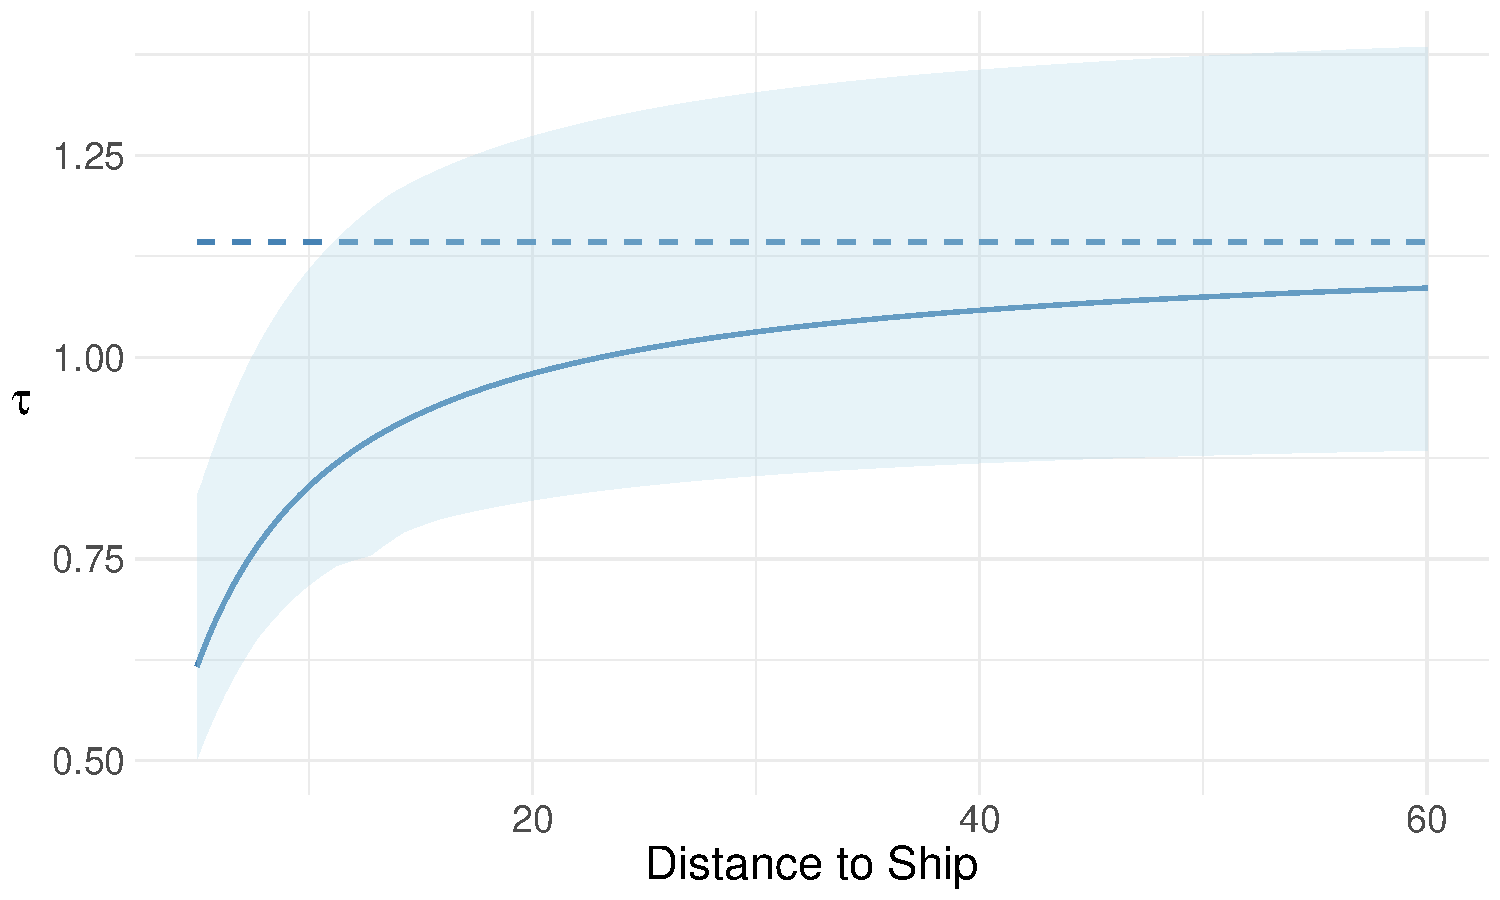
\includegraphics[width=0.7\linewidth]{"images/application/response/fe_tau_ExpShip_final.pdf"}
		\caption{}
	\end{subfigure}
	
	\begin{subfigure}{0.98\textwidth}
		\centering
		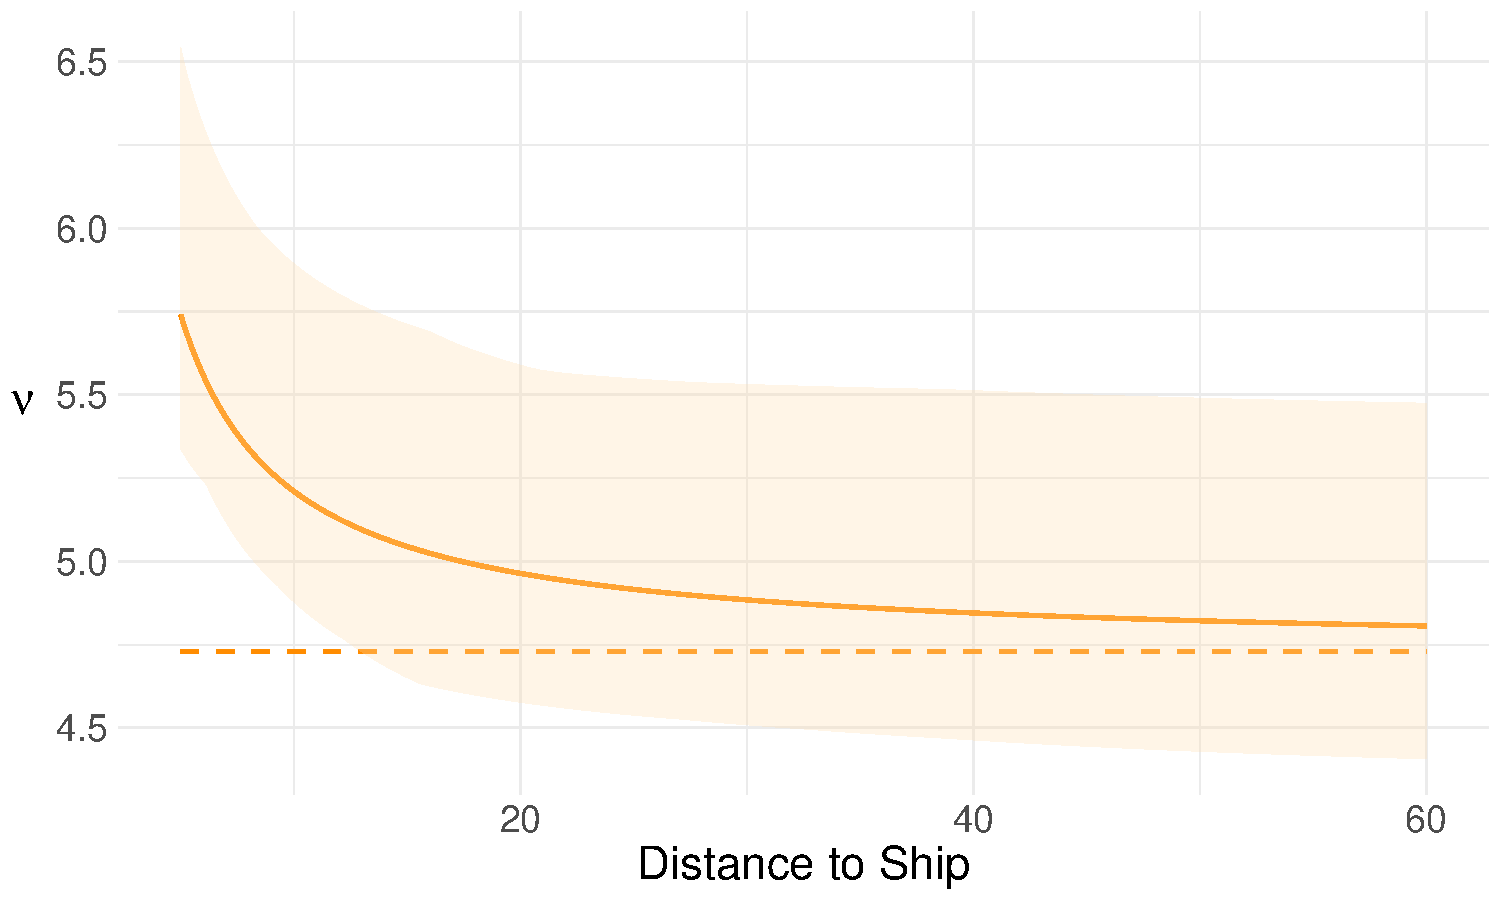
\includegraphics[width=0.7\linewidth]{"images/application/response/fe_nu_ExpShip_final.pdf"}
		\caption{}
	\end{subfigure}
	\caption{Estimated effect of ship exposure on the parameters with $95\%$ confidence intervals. The horizontal dashed lines represent the baseline values. The values on the $x$-axis are in kilometres. (a)  Population persistence parameter $\tau$. Values on the $y$-axis are in hour. (b) Population velocity parameter $\nu$. Values on the $y$-axis are in km/h.}
	\label{fig: population parameters response}
\end{figure}

The distances to the ship $D^{ship}_{\tau}(p)$ and $D^{ship}_{\nu}(p)$  for which a percentage $p$ of deviation from the population baseline values $\tau_0$ and $\nu_0$ are reached are given by 
\begin{equation}
	D^{ship}_{\tau}(p)=\frac{\alpha_{\tau}}{\log(1-p)} \quad  \mbox{and} \quad  D^{ship}_{\nu}(p)=\frac{\alpha_{\nu}}{\log(1+p)}
\end{equation}
Table~\ref{table: recovery_distances} shows these values for different proportions $p$.
For $\tau$, $90\%$ of the baseline value is recovered at a distance about $32$ km. For $\nu$, $110\%$ of the baseline value is reached at a distance about $10$ km. This indicates that sound exposure can be perceived and can disturb the narwhals motion up to tens of kilometres.

Along with other studies, we believe it can serve as a guideline for mitigation measures towards the effects of anthropogenic noise on the narwhals behavior. 

\renewcommand{\arraystretch}{1.75} % Increase row height by 1.5 times

\begin{table}[ht!]
	\centering
	\begin{tabular}{ |c| *{2}{w{c}{10em}|}}
		\hline
		\multirow{2}{*}{Percentage of deviation from baseline} & \multicolumn{2}{c|}{Recovery distance (km) }  \\
		\cline{2-3} 
		& $D^{ship}_{\tau}$ & $D^{ship}_{\nu}$ \\
		\hline
		$50 $ & $4.28 - [2.00,7.13] $&  $2.64 - [1.20,4.25]$ \\
		$10$ & $28.16 -[46.88; 13.18]$ & $11.24 - [5.09; 18.09]$  \\
		\hline
		
	\end{tabular}
	\vspace{0.1cm}
	\caption{Estimated recovery distances of the baseline values within a $50 \%$ and $10\%$ range with $95\%$ confidence intervals.}
	\label{table: recovery_distances}
\end{table}

\subsection{ Baseline model checking}

We use the fitted model to simulate constrained trajectories in the fjords domain with $10$ second time steps.  We then fitted the baseline model on this simulated data. The simulated trajectories from the fitted model before exposure subsampled to $10$ minutes are shown in ~\ref{fig: simulated data} along with the observed data before exposure in figure~\ref{fig: simulated data}. Table ~\ref{table:check_baseline_estimations} shows that we are able to recover pretty well the parameters of the SDE. 

\begin{table}[H]
\centering
\begin{tabular}{lll}
  \hline
Parameter & Estimate & CI \\ 
  \hline
$\tau$ & $1.23$ & $[0.92; 1.61]$ \\ 
  $\nu$ & $4.46$ & $[3.82; 5.18]$ \\ 
  $\sigma_{\tau}$ & $0.22$ & $[0.04; 0.74]$ \\ 
  $\sigma_{\nu}$ & $0.13$ & $[0.04; 0.30]$ \\ 
   \hline
\end{tabular}
\caption{Estimates from simulated trajectories} 
\label{table:check_baseline_estimations}
\end{table}

\begin{figure}
\centering
    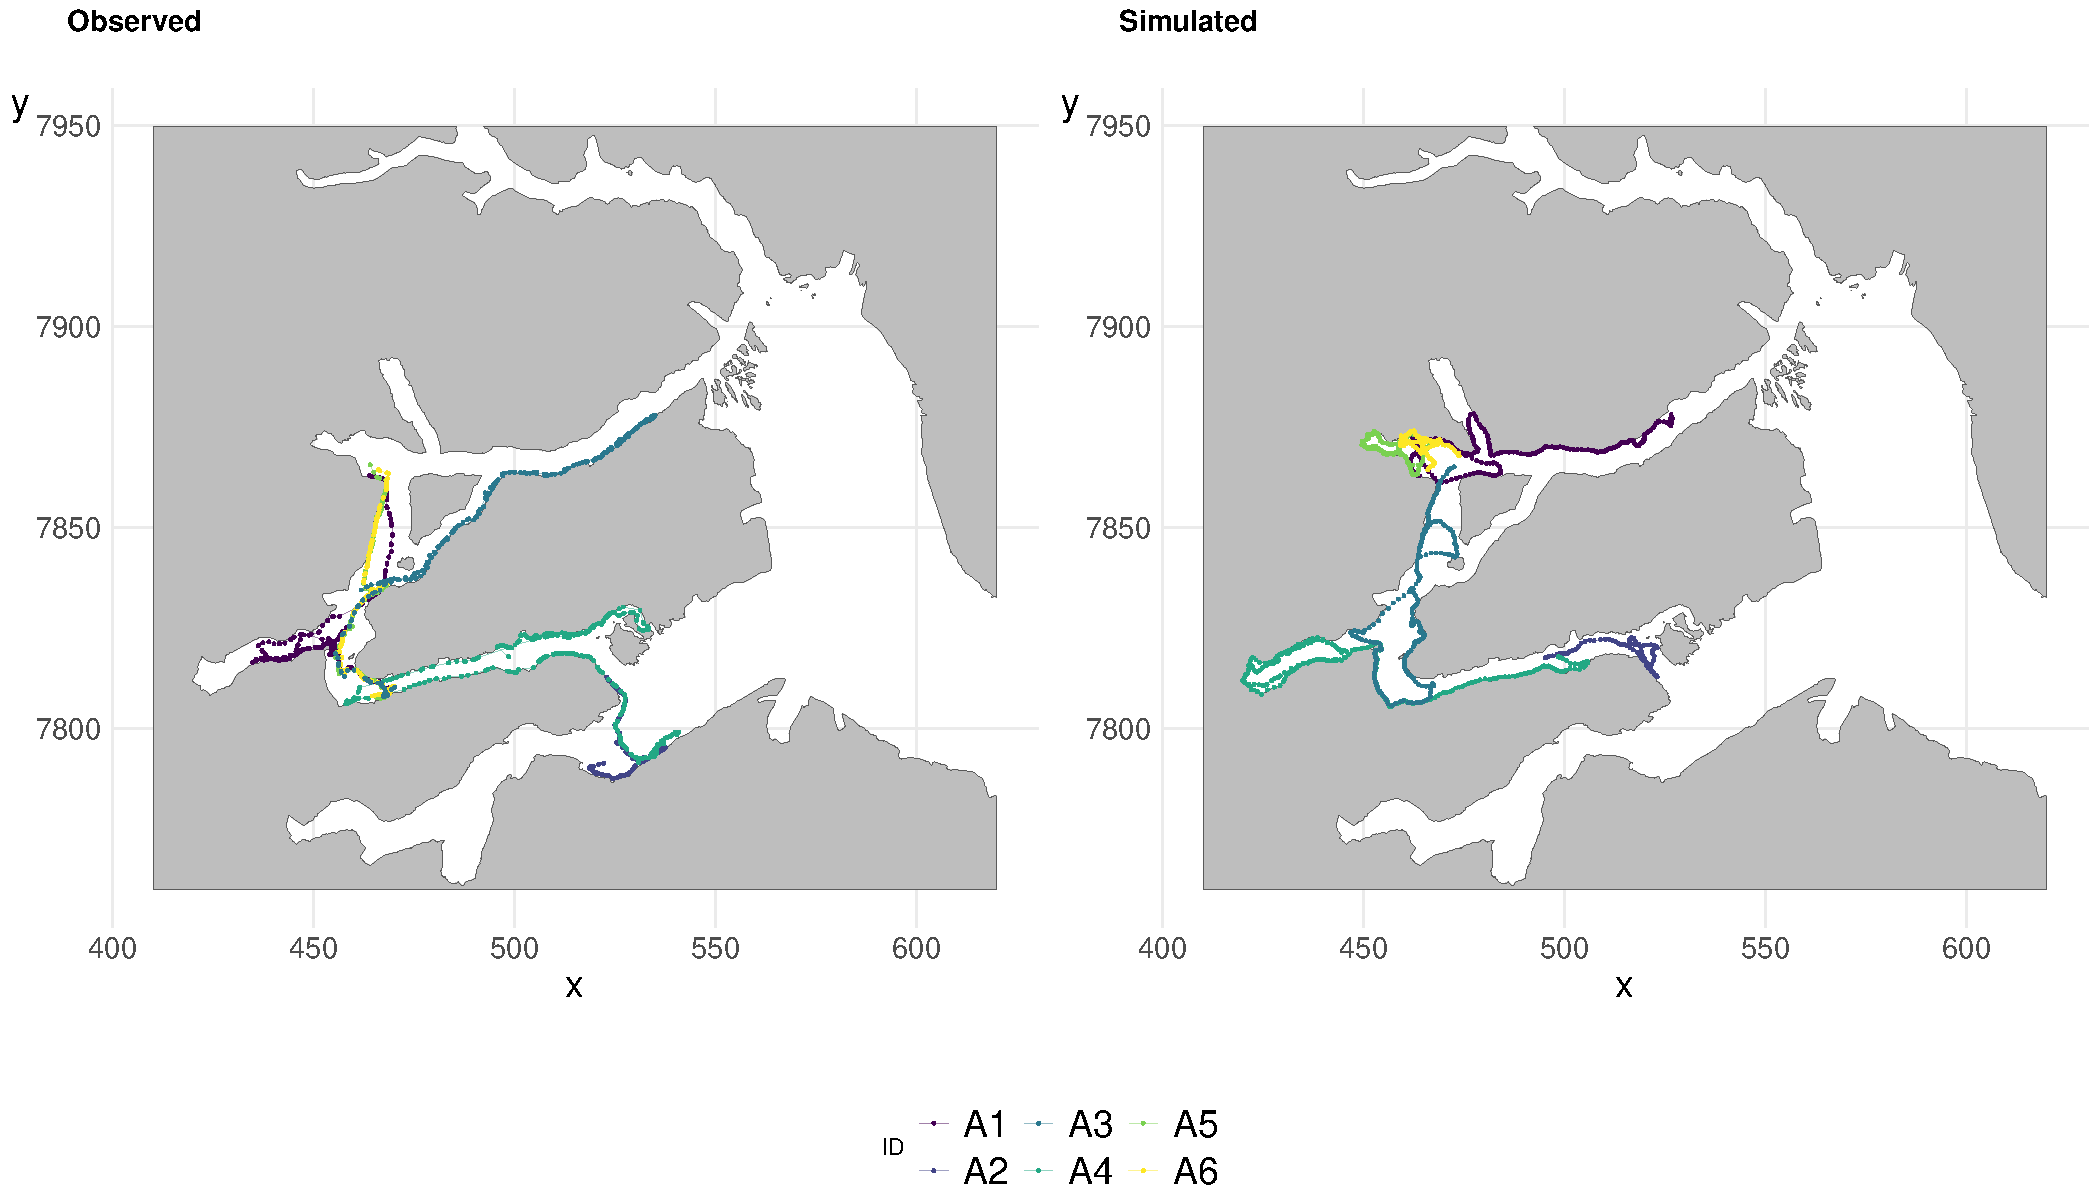
\includegraphics[scale=0.4]{images/application/baseline/plot_baseline_crcvm2_trajectory.pdf}
     \caption{Observed VS simulated trajectories}
    \label{fig: simulated data}
   
\end{figure}

In terms of distance to the shore, observed and simulated data have similar characteristics, which illustrates that our model captures well the space use of the narwhals. We show the histograms of distances to shore for both observed and simulated data in Figure~\ref{fig: Dshore histograms}.


\begin{figure}
\centering
    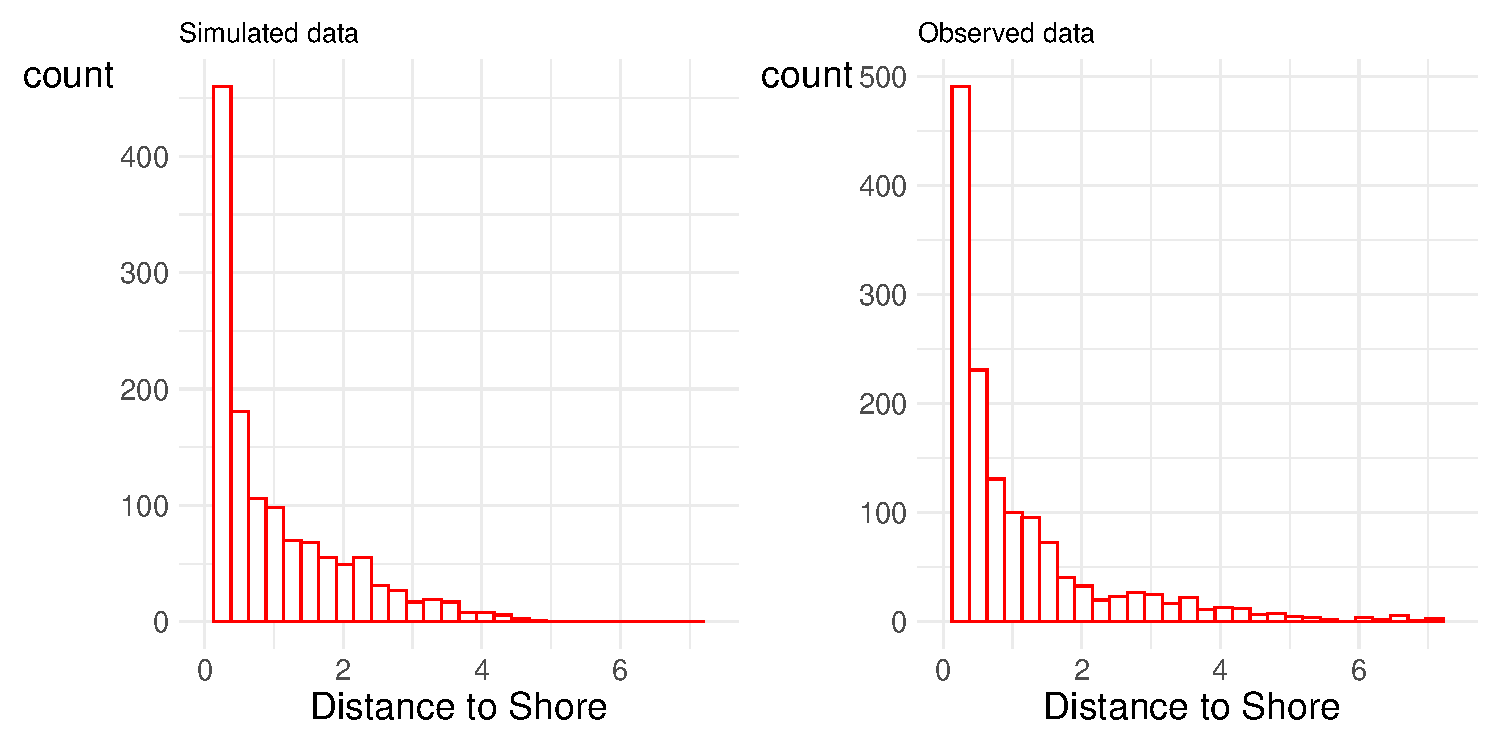
\includegraphics[scale=0.4]{images/application/baseline/Dshore_histograms.pdf}
     \caption{Histograms of distances to shore from observed and simulated data}
    \label{fig: Dshore histograms}
   
\end{figure}


One major difference between the observed trajectories and the simulated ones is that the narwhals have a tendency to move together and follow each other that is not captured in our model. In the data, A5 and A6 as well as A2 and A3 seem to move together for some period of time. We did not include such a behavior in our statistical model.

\section{Conclusion and perspectives}

%summary of the results

We introduced a new method to constrain a stochastic differential equation for animal movement in a bounded region of $\R^2$. Our approach relies on modeling the angular velocity as a function of the distance to the boundary and the angle between the velocity and the boundary normal vector. The additional term that constrains the motion is included in the drift, and, for this reason, acts as a confining potential.
We demonstrated how to simulate such diffusions and how to model different behaviors close to the boundary.\\

This new SDEs with smooth parameters depending on covariates was used to estimate the movement of the narwhals in the fjords. We managed to show an increased tortuosity of the trajectories when approaching the shore. More importantly, we showed that noise exposure has a significant effect on some parameters that drive the motion by comparing a baseline and a response model. We believe this method can be used as a basis for the assessment of behavioral responses in many contexts, and hope it will help understanding better the effects of anthropogenic noise on marine mammals movement.

We emphasize that, even if we were able to estimate quite reliably the smooth parameters of the SDE, a part of uncertainty still remains. First, the log-likelihood function that we rely on for the estimation is approximate, based on piecewise constant parameter values on each time step. Given that observations are relatively high frequency (5 min between consecutive observations in median), the error introduced is expected to be low, though we don't have theoretical bounds for it. Moreover, the constant covariate value that is used on each time step is computed from the GPS observations, even though these observations come with GPS measurement error. We don't integrate the measurement error in the covariates $\Theta$, $E^{ship}$ and $I^{shore}$ that we are considering. Since GPS measurement error are pretty low (a few tens of metres) compared to ARGOS for instance, this may not introduce significant error in the estimations. Eventually, Laplace approximation is used to approach the integral of likelihood over the random effects. We did not discuss the error that may be introduced by this approximation, but the simulation study show that despite all the approximations made along the way, we are indeed able to get reliable estimates even for pretty complex models.\\

In the future, studying theoretical properties of the SDE models we used here might be of significant interest. For instance, we did not prove any result or exhibit clear assumptions that would guarantee that the process is effectively constrained. We noticed that in the literature of animal movement modeling, whether that would be with SDEs, HMM or step-selection functions, spatial constraints are rarely considered. We hint that better considerations of the spatial constraints can give new insights into the interactions between marine mammals and their environment.


%%%%%%%%%%%%%%%%%%%%%%%%%%%%%%%%%%%%%%%%%%%%%%
%% Support information, if any,             %%
%% should be provided in the                %%
%% Acknowledgements section.                %%
%%%%%%%%%%%%%%%%%%%%%%%%%%%%%%%%%%%%%%%%%%%%%%


%%%%%%%%%%%%%%%%%%%%%%%%%%%%%%%%%%%%%%%%%%%%%%
%% Funding information, if any,             %%
%% should be provided in the                %%
%% funding section.                         %%
%%%%%%%%%%%%%%%%%%%%%%%%%%%%%%%%%%%%%%%%%%%%%%
\begin{funding}
% The first author was supported by ...
The authors would like to thank the CNRS and IRN Madef for funding A. Delporte, and MIAI - ANR-19-P3IA-0003 for the funding of A Samson.
We also thank the project MATH-AmSud 23-MATH-12.
% The second author was supported in part by ...
\end{funding}

%%%%%%%%%%%%%%%%%%%%%%%%%%%%%%%%%%%%%%%%%%%%%%
%% Supplementary Material, including data   %%
%% sets and code, should be provided in     %%
%% {supplement} environment with title      %%
%% and short description. It cannot be      %%
%% available exclusively as external link.  %%
%% All Supplementary Material must be       %%
%% available to the reader on Project       %%
%% Euclid with the published article.       %%
%%%%%%%%%%%%%%%%%%%%%%%%%%%%%%%%%%%%%%%%%%%%%%
\begin{supplement}
\stitle{Shapefile for land geometry}
\sdescription{Shapefile based on OpenStreetMap data for the land polygons in Scoresby Sound fjords system. We used high resolution satellite images to improve it with \texttt{qgis} software and applied a geometric buffer of $100$ metres.}
\end{supplement}

%%%%%%%%%%%%%%%%%%%%%%%%%%%%%%%%%%%%%%%%%%%%%%%%%%%%%%%%%%%%%
%%                  The Bibliography                       %%
%%                                                         %%
%%  imsart-nameyear.bst  will be used to                   %%
%%  create a .BBL file for submission.                     %%
%%                                                         %%
%%  Note that the displayed Bibliography will not          %%
%%  necessarily be rendered by Latex exactly as specified  %%
%%  in the online Instructions for Authors.                %%
%%                                                         %%
%%  MR numbers will be added by VTeX.                      %%
%%                                                         %%
%%  Use \citep{...} to cite references in text.             %%
%%                                                         %%
%%%%%%%%%%%%%%%%%%%%%%%%%%%%%%%%%%%%%%%%%%%%%%%%%%%%%%%%%%%%%

\bibliographystyle{imsart-nameyear} % Style BST file
\bibliography{aoas-template}       % Bibliography file (usually '*.bib')
\end{document}
